%!TEX root = thesis.tex

A lot of things jam; cars do it in traffic, musicians do it during a rehearsal, paper does in printers, and we might even put it on bread.
In this chapter particles jam.
\blank
As mentioned in our definition of AHIs in \autoref{ch:adhoc} we proposed three different approaches to creating AHIs.
In this chapter we will explore the first approach which was to use shape-change as a construction mechanism for AHIs.
So in this chapter we will dig in to the area of shape-changing interfaces to explore and illustrate the possibilities of creating AHIs based on shape-change.
More specifically we will touch upon a specific approach to constructing SCIs called jamming.

SCIs were introduced in the introduction of this thesis as interfaces that use physical change of shape as input or output.
Jamming is special kind of technique that can be used to control the stiffness of a material which makes it possible to construct objects that can change their surface structure.

What makes SCIs interesting to AHIs is it's ability to dynamically change the physical properties of an interface element, be it shape, texture, stiffness, position ect.
This change in physicality can then be the offset for a new temporary interaction possibility that is created for the specific situation, where afterwards it can return to it's initial natural state.
Compared to TUIs, SCIs have the ability to form a dynamic relationship between the physical objects and the digital state of the system, allowing both the user and the computer to change the physical state of an object to match its digital state.
These aspect aligns well with the definition of AHIs that we presented earlier in section~\ref{adhoc:definition}.
\blank
The process of our exploration of SCIs has, at times, been somewhat discouraging as we have proceeded to learned the lessons of the difficulty of creating such interfaces.
We have come to the conclusion that SCIs are indeed non-trivial to build and prototype, a lesson that we think everyone who has worked on SCIs must have experiences at some point, although it has not been widely mentioned in the literature. 

There are some inherently difficult aspects of creating objects with kinetic movements, for example in our earlier described BeoMotion project the change from flat surface to edged surface proved difficult as the phase change, because we worked with non-elastic materials, caused a contraction of the base structure.
We solved this by putting small rails on each of the individual elements of the structure to allow the contraction but this caused a new problem as small gaps now emerged since the base of the elements was able to move sightly in relation to each other.

In our exploration of jamming we also ran in to various problems.
While we consider ourselves fairly home in physical computing we, perhaps a little overconfident, initially thought it would be moderately straight forward to build pneumatic and hydraulic jamming systems.
We quickly ran into difficulties though with a seemingly continuous stream of new challenges in relation to vacuum pumps, compressors, solenoid valves, custom made membranes, various fittings and connectors between non-fitting tubes, particles and filters -- all elements that we had never worked with before, see figure \ref{fig:ch:jamming:materials}.
On top of that all of these pieces had to work together while being air or water tight. 

So while we did not end up with a finished, ready-to-test prototype we did still, in our opinion, gain relevant experiences and additions to our notion of AHIs, in the shape of concrete experience with building AHIs, concept development and a study of the field of jamming and its relevance to AHIs. 

\begin{figure}[h]
	\centering
	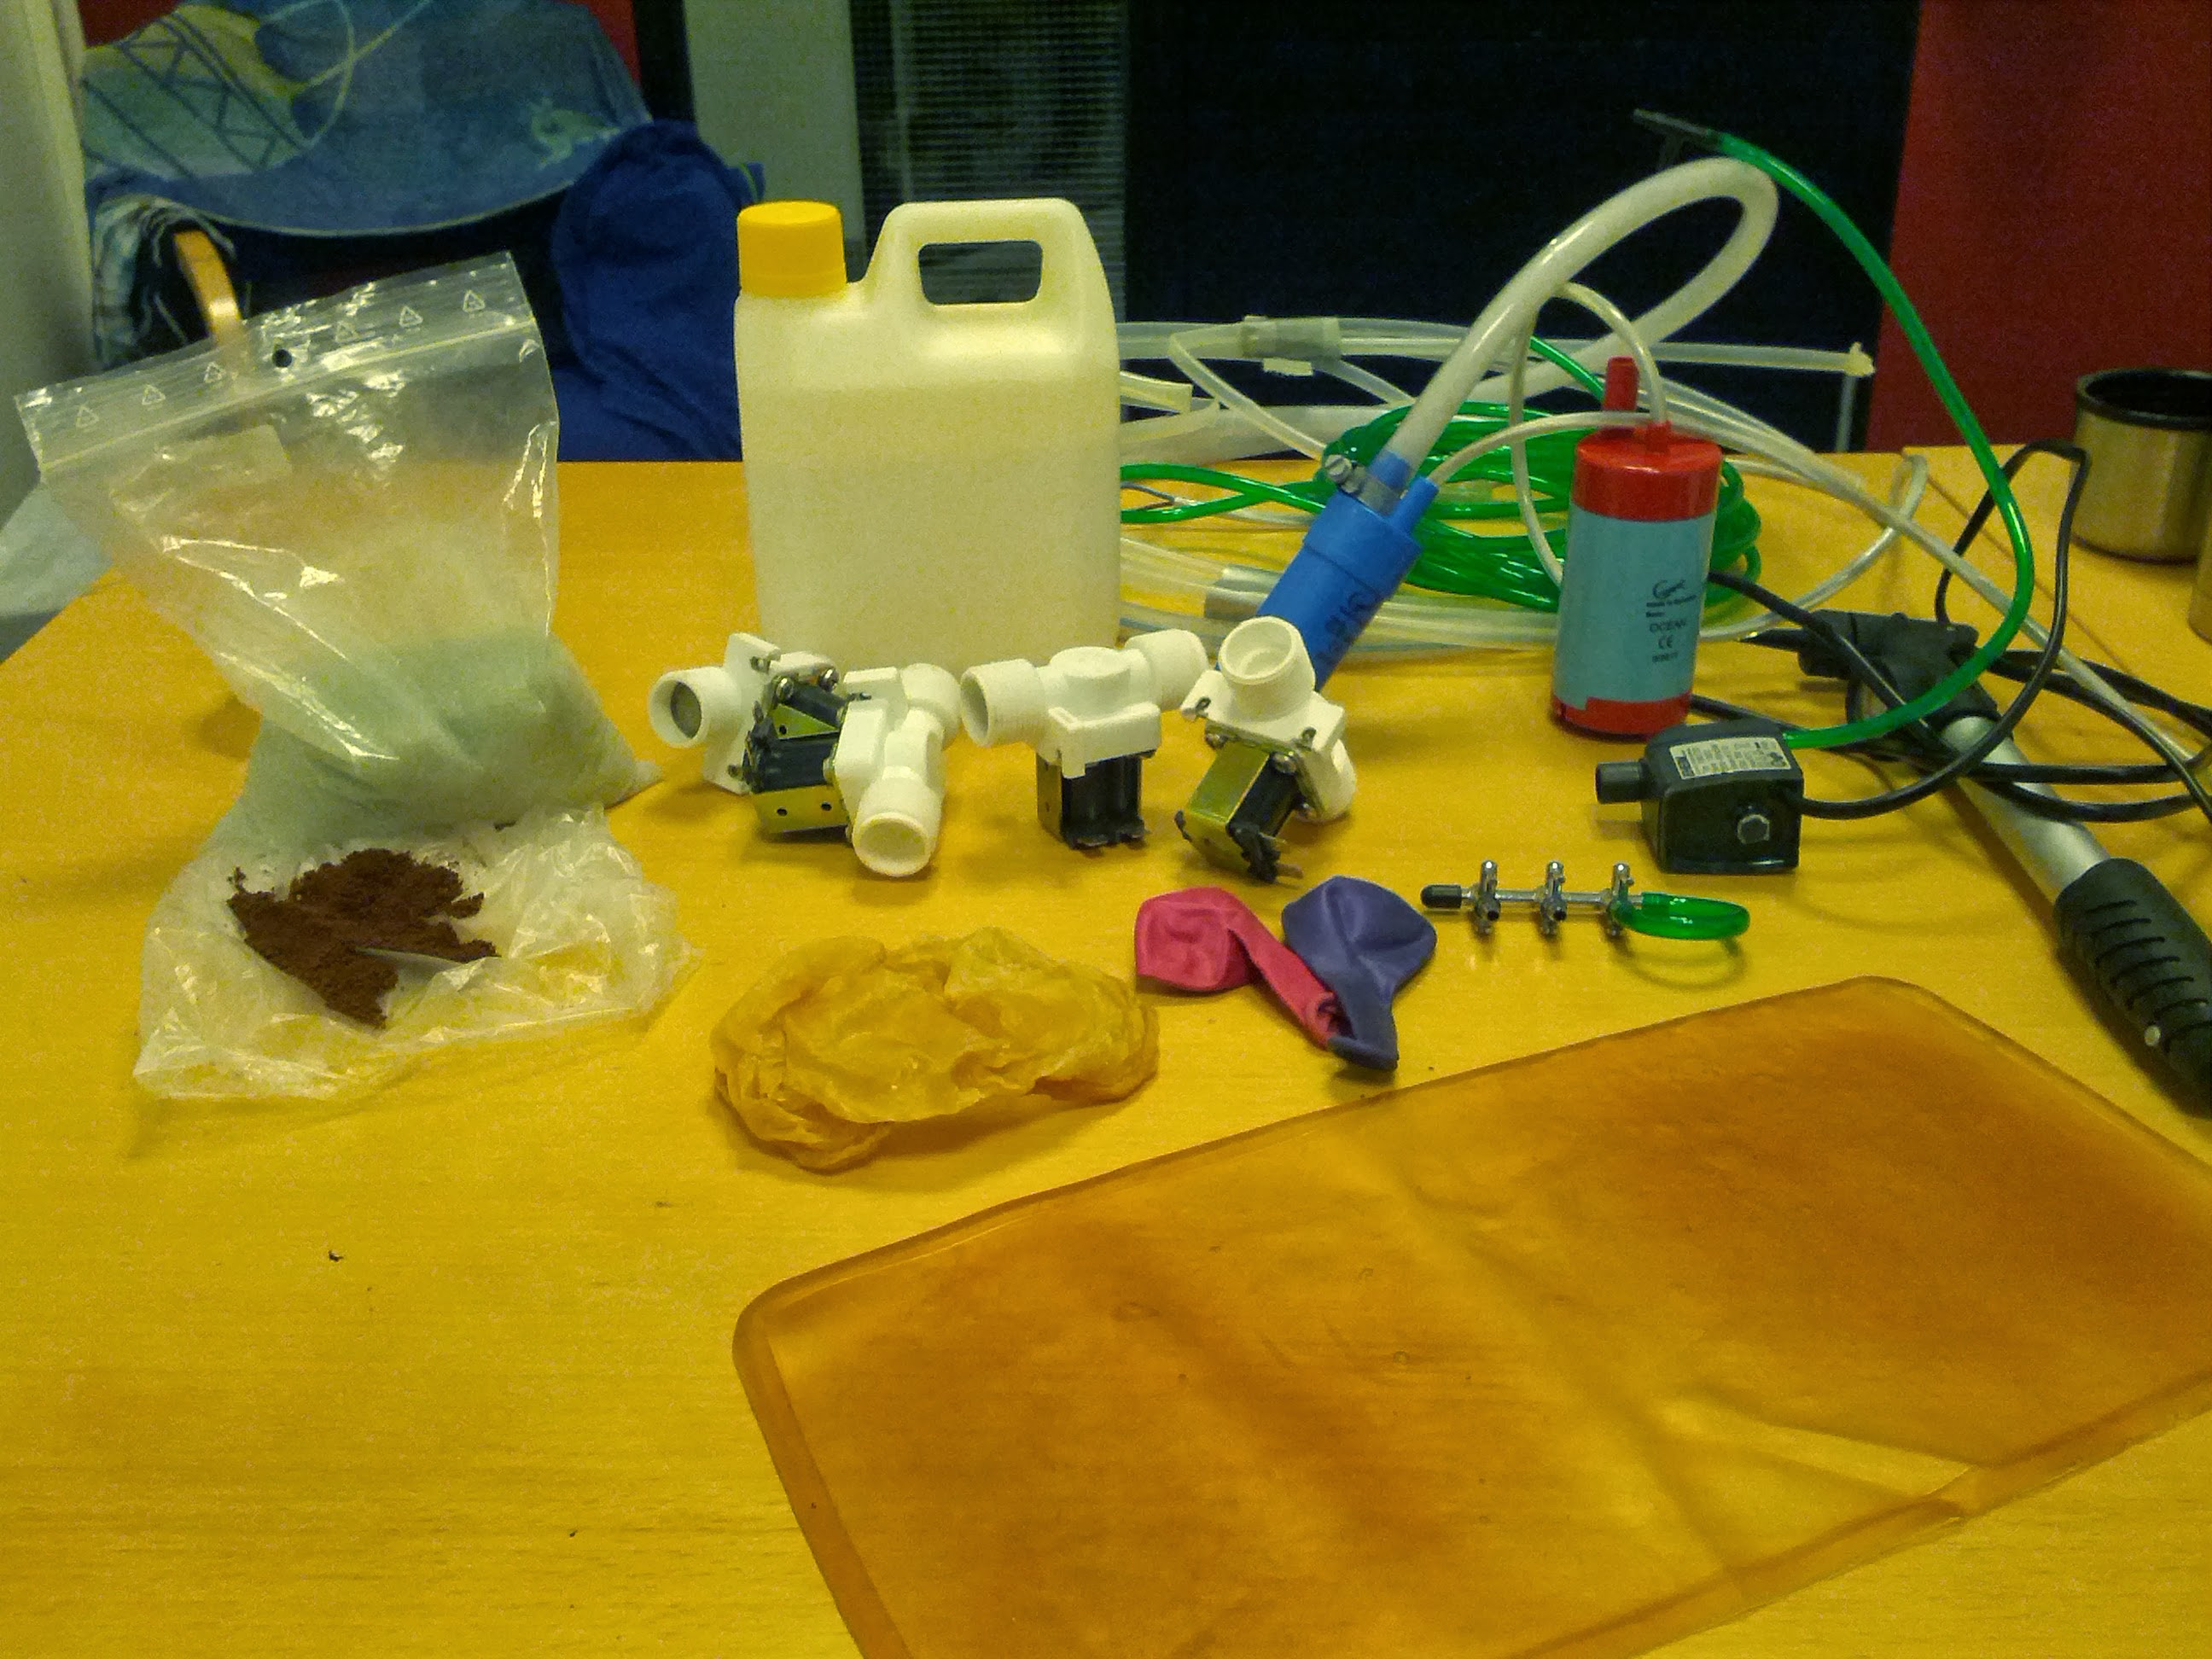
\includegraphics[width=.9\linewidth]{figures/jamming/jamming-materials}
	\caption{A selection of the materials we acquired and used for a jamming system. \textbf{Far left:} glass-beads and ground coffee which were used as granular material. \textbf{Front:} custom membranes made from rubber milk (white container in background) and balloons. \textbf{Center:} white solenoid valves for electronic control of the flow of fluid and a manual valve next to the balloons. \textbf{Right:} three different electronic pumps for moving fluids and lastly a manual pump.}
	\label{fig:ch:jamming:materials}
\end{figure}

\section{A vocabulary of shape-change}
\label{ch:jamming:shape-change} 
%!TEX root = ../thesis.tex
\todo{more introduction, back-reference to chapter 3}

\todo{SCI chapter needs review to make it more relevant to the prototyping}

Shape-changing interfaces (SCIs) are a relative new subject in the area of human-computer interaction.
In previous work it has been discussed under various different terms such as Kinetic Interaction, Organic User Interfaces, Actuated Interfaces, to name a few stated by \citet{rasmussen2012shape}.

\subsection{A vocabulary of shape-change}
\label{ch:jamming:vocabulary}
In this chapter we will expand our vocabulary regarding SCIs based on \citet{coelho2011shape} and \citet{rasmussen2012shape}.
They both provide contributions as to how we can talk about SCIs, how we can group and identify different types of change of shape, how we can identify and describe shape transformations, and most importantly, how and to which purpose we can interact with SCIs.
We will use this vocabulary onwards in our thesis to discuss SCIs, both ours and others.   
Rasmussen defines shape-changing interfaces as
\begin{quotation}
  \emph{A shape-changing interface uses physical change of shape as input or output.}
\end{quotation}
and further
\begin{quotation}
  \emph{[\ldots] the self-actuation must be controllable so that the object can return to its initial state and repeat the shape change. }  
\end{quotation}

\citeauthor{coelho2011shape} presents a grouping which distinguish three types of change of shape: \emph{topological, textural and permeable} transformations.
Topological transformations here being those transformations which adhere to topological equivalence, permeable those which do not and textural transformation stands as a category for it. Topologically equivalence here means that a form can transform in to another form by a continuously homeomorphic transformation - that is without cutting or gluing either form. This can be exemplified by the pliable donut that transforms into a coffee mug without breaking homeomorphism as seen in figure~\ref{pliable-mug} \todo{lav egen figur?} 

\begin{figure}[hb]
	\centering
  		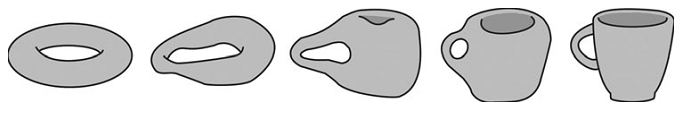
\includegraphics[width=4in]{figures/pliable-donut}
	\caption[The pliable donut momeomorphic transformation, taken from \citep{coelho2011shape}]
   {The pliable donut momeomorphic transformation, taken from \citep{coelho2011shape}}
   \label{pliable-mug}
\end{figure}   
 
\citeauthor{rasmussen2012shape} suggests a grouping more detailed grouping of shape-changing interfaces by identifying eight types of change of shape, namely: \textit{orientation, form, volume, texture, viscosity, spatiality, adding/subtracting and permeability}.
These eight fit into two groups where the first six are topologically equivalent and the last two are not. This is in line with what \citeauthor{coelho2011shape}, though texture standing has been moved into the topologically equivalent group. Overall it expands on \citeauthor{coelho2011shape}s work and enables us to identify and discuss form changes in more detailed terms.
The grouping is visualized in figure~\ref{types-of-change}, illustrating the different types of change.

\begin{figure}[hb]
	\centering
  		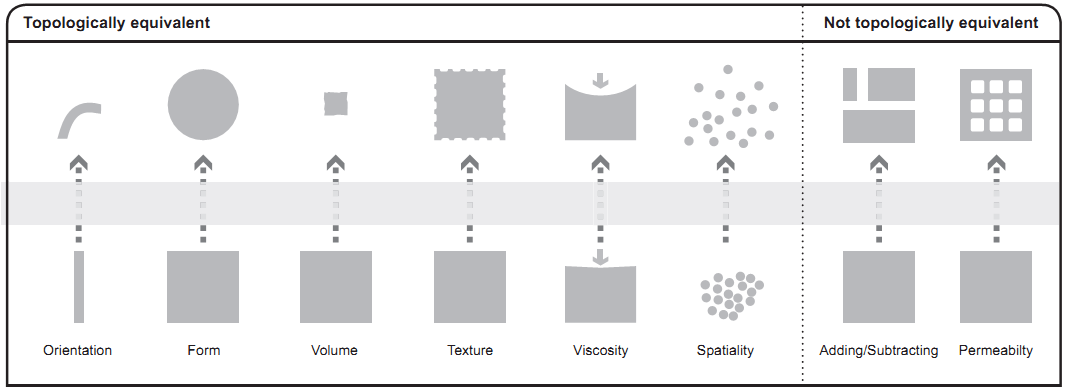
\includegraphics[width=4in]{figures/types-of-change}
	\caption[Types of shape-change as visualised by \citep{rasmussen2012shape}]
   {Types of shape-change as visualised by \citep{rasmussen2012shape}}
   \label{types-of-change}
\end{figure}

There might be some debatable cases in this grouping, e.g. they define textural change as
\begin{quotation}
small changes on the surface of the shape that add visual and tactile properties without affecting the overall form
\end{quotation} 
so if the overall form is not changed it might not make sense to classify it as a homomorphic transformation, which might also be the reason why \citeauthor{coelho2011shape} chose to separate it as a case for itself.
Also if we look at the case of spatiality changes where a collection of elements form a single object, it is possible to think of examples where non-homeomorphic transformations occurs if, for example, the collection of elements split in the middle forming two objects and then merge back together.
This would still count as a shape-changing interface as described in the definition but would not adhere to topological equivalence.   

The transformation in itself is interesting as well and \citeauthor{rasmussen2012shape} reveals different types of transformation.  They describe the transformation as the \textit{phase between endpoints}, meaning the phase between the form's origin and its morphed state.
They distinguish between kinetic parameters and expressive parameters, where
the kinetic parameters describe the physical movements of the transformation and the expressive parameters relates to how the kinetic movements are perceived and understood.
This is a very interesting and important aspect of SCIs since it, together with the theory of affordances, provides the basis for understanding the interface and its functions, which at the same time is one of the key challenges of SCIs.
Since SCIs are inherently non-static objects we might not be able to rely on the form alone to communicate the intent and functions of the object, so there might have to be some interaction clues elsewhere, for example in the transformation itself. This will be discussed in more detail in chapter \todo{ref somewhere}  

A key aspect of SCIs, and any user interface in general, is the interaction - be it direct physical interaction, implicit visual interaction, or something in between. 
\citeauthor{rasmussen2012shape} distinguish between \textit{no interaction}, where there is only shape-changing output; \textit{indirect interaction}, still only with shape-changing output but based on implicit user input; \textit{direct interaction}, where the user deforms the object in some way as user input and a shape-change output occurs, either in the object itself or in a remote object.
Two approaches to direct interaction are identified, \textit{action and reaction} where the object reacts directly to the action in a synchronized process and \textit{input and output} where the object is acting asynchronously and not necessarily directly related to the input.    
Our focus will be on objects with direct interaction and mainly those with input and output merged into the same object, as we here see the best possibilities for creating interfaces \todo{et eller andet}
 
\hl{Our own exploratory work will focus only on topological transformations, excluding spatiality, since our choice of technology hinders this type of change.} This will be further described in section \todo{ref til proto 0}  

\section{Jamming as an enabling technology}
\label{ch:jamming:enabling-technology} 
%!TEX root = ../thesis.tex
Before continuing on the topic of jamming, let's first give an introduction to the mechanics of jamming.

Jamming is a mechanism that can enable granular material to transition between solid-like and liquid-like states. These states can occur if the material is put under an external stress, figure~\ref{fig:ch:jamming:phase-transition} illustrate these states.
Much like water can shift to gas when heated and to ice when cooled. But where water is affected by thermodynamics, granular systems are not. \hl{entirely true?}
Sand, which is a granular material, may resemble a liquid as it flows through an hour glass, although the individual grains themselves are a solid structure. This is due to something called \todo{Jamming, Force chains and Fragile matter}

\begin{figure}[hb]
	\centering
  		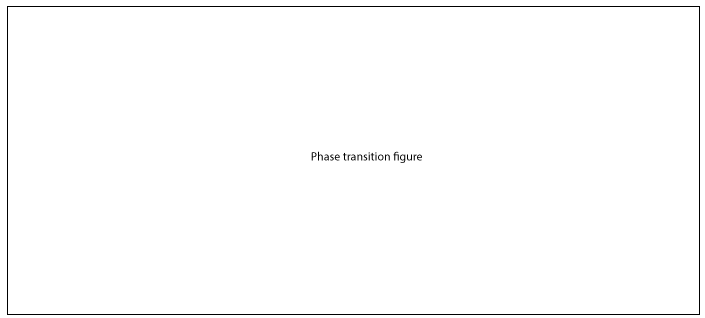
\includegraphics[width=4in]{figures/jamming/phase_transition}
	\caption[Phase transition from \textit{liquid} state to \textit{solid} state.]
   {Phase transition from \textit{liquid} state to \textit{solid} state.}
   \label{fig:ch:jamming:phase-transition}
\end{figure}

You might have noticed how some coffee packagings at the local super market are like a rigid container, see figure~\ref{fig:ch:jamming:coffee-packaging}. 
In this kind of packaging, after filling it with coffee, all excess air has been sucked out by applying a vacuum, i.e. jamming the coffee grains, and thereby making it almost rock solid. 
Also, think about a regular bean bag which exhibits some of the same properties, see figure~\ref{fig:ch:jamming:bean-bag}. 
When no force is applied to it, i.e. no one is sitting in it, it resembles the liquid-like state mentioned earlier. 
When a person then sits down in a bag air will be pressed out and the particles (most often polystyrene foam) will be pushed tightly together filling the voids  \todo{some physical term here, phase space and stuff} thereby jamming the particles making it resemble a solid ...

\begin{figure}
\centering
\begin{minipage}[t]{.5\textwidth}
  \centering
  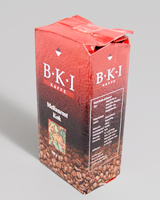
\includegraphics[width=.4\linewidth]{figures/jamming/coffee_packaging}
  \captionof{figure}{Coffee in vacuum packaging}
  \label{fig:ch:jamming:coffee-packaging}
\end{minipage}%
\begin{minipage}[t]{.5\textwidth}
  \centering
  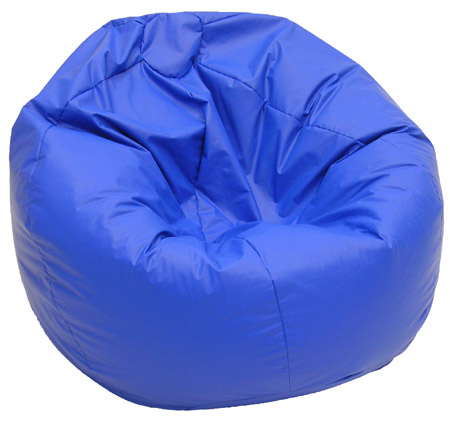
\includegraphics[width=.4\linewidth]{figures/jamming/bean_bag}
  \captionof{figure}{A bean bag}
  \label{fig:ch:jamming:bean-bag}
\end{minipage}
\end{figure}

\subsection{Particles}
\label{ch:jamming:particles}
The granular material, also called the particles, can be any material that has the physical properties that allow for jamming to occur. 
But parameters such as particle size, shape and compressibility have an impact on the jamming transition. 
This has been investigated by several researchers, e.g. \cite{cheng2012design} and \cite{steltz2010jamming}, where the stress to strain ratio \todo{explain this} of different granular materials are evaluated. 
Ground coffee (fine and coarse) and glass beads of varying size are recurring across these tests, the first being an irregular shape with a rough surface as opposed to the plain shape and smooth surface of the second, see figure~\ref{fig:ch:jamming:particles-close-up}. 
Particles of same size and with a smooth surface will tend to be more fluid-like when unjammed as they flow more freely. 
Irregular particles with rough surfaces will create more friction between the particles thus being less fluid-like in the unjammed state.

The conclusion is that the choice of granular material is very much dependent on the application in question. 

\begin{figure}
\centering
\begin{subfigure}{.5\textwidth}
  \centering
  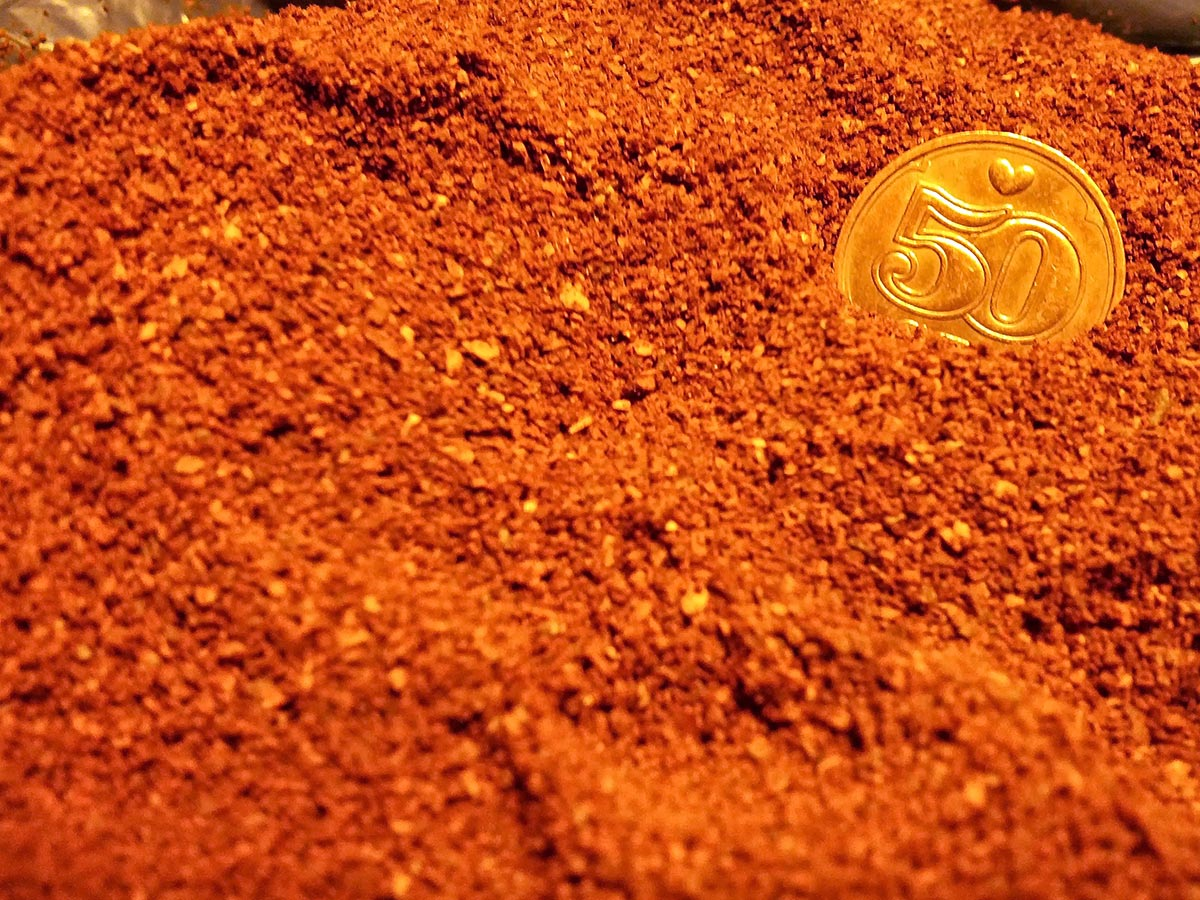
\includegraphics[width=.9\linewidth]{figures/jamming/coffee-grains}
  \caption{Grounded coffee}
  \label{fig:sub1}
\end{subfigure}%
\begin{subfigure}{.5\textwidth}
  \centering
  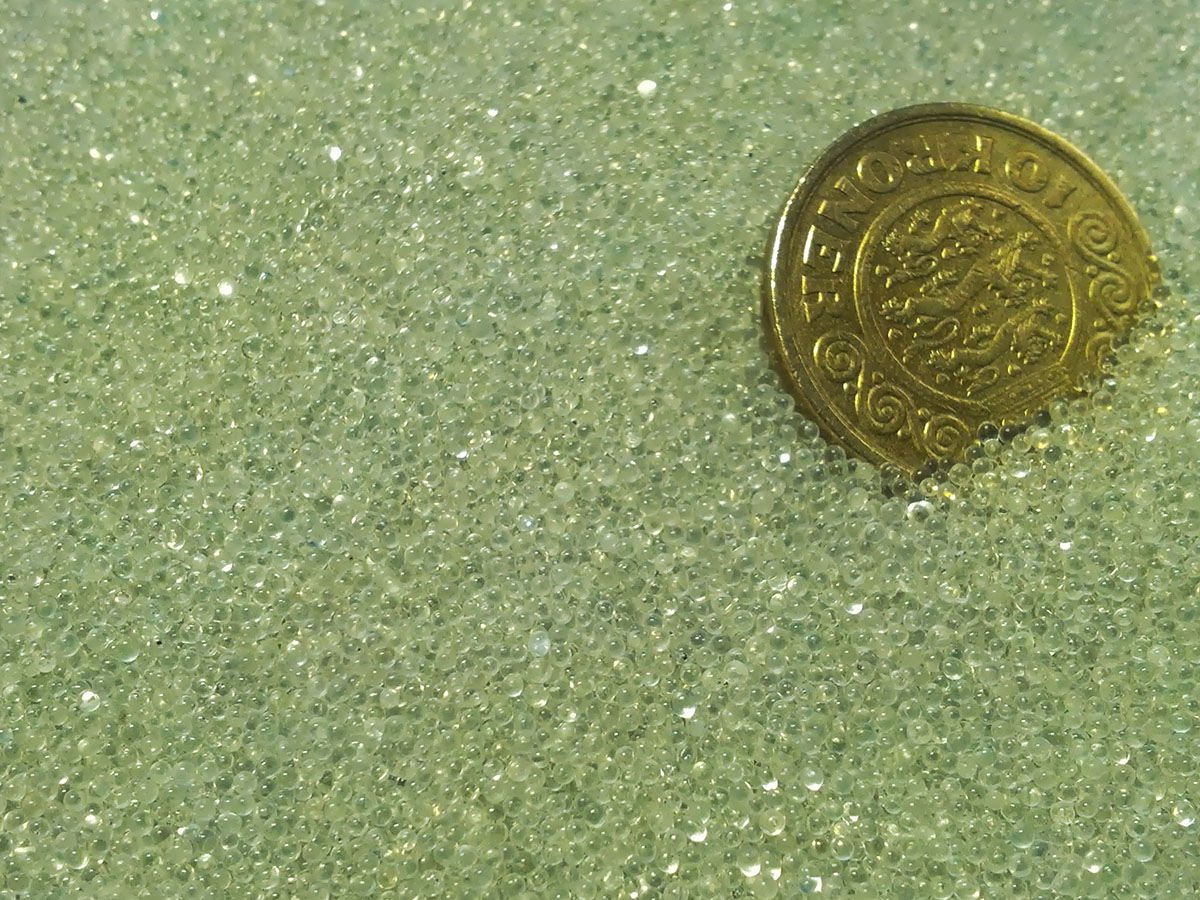
\includegraphics[width=.9\linewidth]{figures/jamming/glass-beads}
  \caption{Glass beads}
  \label{fig:sub2}
\end{subfigure}
\caption{A microscopic view of different granular material.}
\label{fig:ch:jamming:particles-close-up}
\end{figure}

\todo{research in particle parameters in other\\ disciplines such as robotics.}

\begin{itemize}
	\item http://en.wikipedia.org/wiki/Jamming\_(physics)
	\item http://www.nature.com/nphys/journal/v3/n4/full/nphys580.html
	\item http://www.nature.com/nature/journal/v411/n6839/full/411772a0.html
\end{itemize}

\subsection{The technique}
\label{ch:jamming:technique}

The jamming technique can be applied with both a pneumatic and a hydraulic approach.
In the pneumatic approach a gas, for example air, is used as a means for actuation, see figure~\ref{fig:ch:jamming:jamming-basics}.
The gas is enclosed together with granular material within a flexible and air tight container, for example rubber latex. 
A filter prevents the granular material from escaping the container and a valve upholds the pressure.
An external vacuum pump can then suck out the air of the container, creating a negative pressure inside, which results in the transition to a solid-like form. 
The speed of this transition of course depends on the suction power of the pump.
When the vacuum is released the form will gradually transition back to the liquid state. 
In this way, the transition allows for states in between the two extremes; solid and liquid.

Jamming makes it possible to deform an object by hand while in the liquid state and then apply the vacuum and make the deformed object solid - in a sense the form is \emph{saved} as long as the vacuum is maintained.
Figure~\ref{fig:ch:jamming:jamming-transition} shows a transition where a form has been molded and solified into a shape.
When the pressure is released the form gradually changes shape as seen in the individual steps of the figure.
In the setup a balloon was used as the membrane and ground coffee within as particles.
Pressure was applied with a vacuum cleaner and a coffee filter prevents the particles from being sucked out.

In the example it can be seen that the object (balloon) returns to its initial state which is a requirement for SCIs as stated earlier in section \ref{ch:jamming:vocabulary}.
In this example it is the tension of the latex of the balloon that forces it back but it could as well have been an actuation done with the jamming technique itself. 

\begin{figure}[hb]
	\centering
  		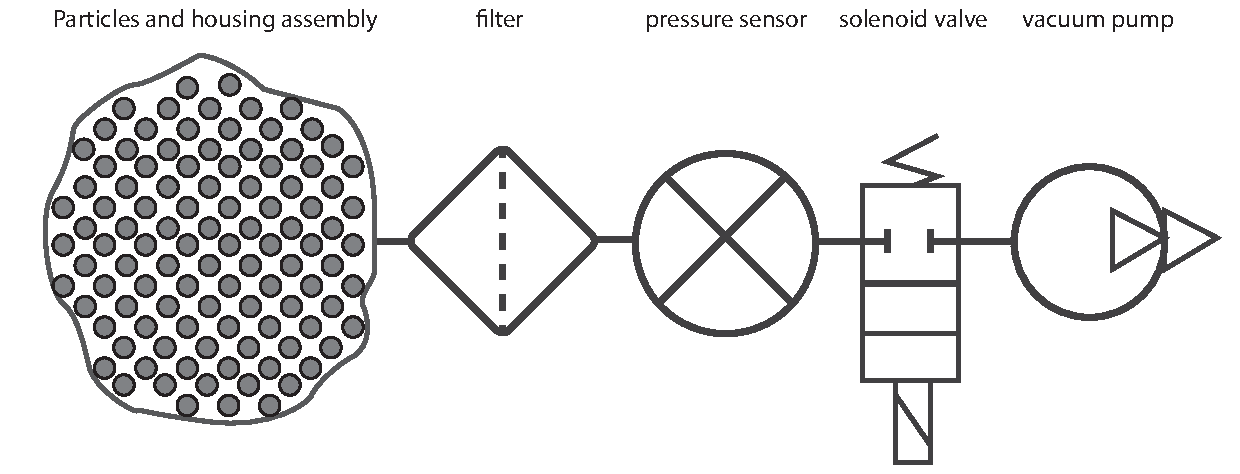
\includegraphics[width=4in]{figures/jamming/jamming-basics}
	\caption[A basic pneumatic jamming system.]
   {A basic pneumatic jamming system.}
   \label{fig:ch:jamming:jamming-basics}
\end{figure}

\begin{figure}[hb]
  \centering
      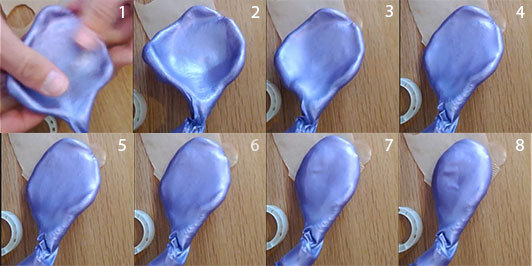
\includegraphics[width=\textwidth]{figures/jamming/jamming-transition}
  \caption[A jamming transition setup.]
   {Jamming transition with a balloon, grounded coffee, vacuum cleaner and a coffee filter.}
   \label{fig:ch:jamming:jamming-transition}
\end{figure}



\section{Related work}
\label{ch:jamming:related-work} 
%!TEX root = ../thesis.tex
Although jamming might seem as a novel approach in the area of HCI, other areas of research have had it on their agenda for some time. 
Especially in the area of mechanical engineering where the jamming mechanism has shown promising results in robotic applications as a substitute for mechanical parts.
In the following we cover the current applications of jamming in both HCI and engineering. 

\subsubsection{Mechanical engineering and robotics}

\citet{brown2010universal} and \citet{amend2012positive} used the jamming technique to develop a universal robotic gripper, which is the tool at the end of a robotic arm that interacts with its environment.
This is an example of the basic jamming approach with a single volume, as in figure~\ref{fig:ch:jamming:approaches:basic}.
The gripper was simply built with an elastic bag as a container for the granular material, which was chosen to be grounded coffee. 
It is able to pick up objects of heterogeneous shapes due to the gripper simply adapting to the surface structure of the objects on impact, see figure~\ref{fig:ch:jamming:jamming-robot-gripper}. 
Contrasting this with a normal mechanical robotic arm which needs several actuators to grap objects of heterogeneous shapes, this gripper is implemented with a single actuator, the jamming volume, which still obtains multiple degrees of freedom (DoF).

\begin{figure}[h]
  \centering
  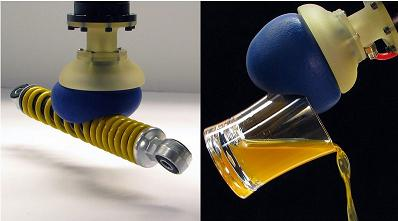
\includegraphics[width=0.9\linewidth]{figures/jamming/jamming-robot-gripper}
	\caption[A universal robotic gripper based on the jamming of granular material by \citet{brown2010universal}.]
   {A universal robotic gripper based on the jamming of granular material \citep{brown2010universal}.}
   \label{fig:ch:jamming:jamming-robot-gripper}
\end{figure}

Jamming is also seen in experiments with autonomous robots where the mechanism can be used as artificial muscles.
\citet{steltz2009jsel} used the jamming technique to create a platform for shape-changing and mobile robots called JSEL (Jamming Skin Enabled Locomotion).
As opposed to the previous example this work is based on the cell-based jamming approach, as seen in \ref{fig:ch:jamming:approaches:cell}.
The soft robot can morph its ``skin'' to create movement of the entire body by controlling the stiffness of the individual cells and inner actuator (see figure~\ref{fig:ch:jamming:jsel}). 

\citet{steltz2010jamming} took the JSEL approach further combining the cell-based approach with a linear actuator. 
The assembly combines the contraction and extension capabilities of the linear actuator and modulates this 1-DoF actuation into a multi-DoF actuator depending on the number of surrounding jamming cells.
The platform is called JMU (Jamming Modulated Unimorph) and has been tested as component segments of a worm, as an example of a soft robot (see figure~\ref{fig:ch:jamming:jmu}).

These different examples from other fields of research illustrate how creative implementations of the jamming technique can substitute mechanical parts and in many ways simplify the implementation.

\begin{figure}
  \centering
  \begin{minipage}[t]{.44\textwidth}
    \centering
    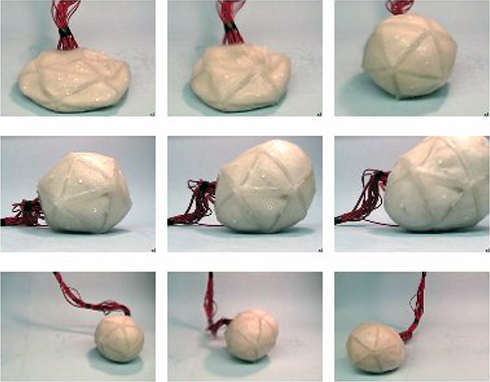
\includegraphics[width=\linewidth]{figures/jamming/chembot-robot-blob}
    \caption[Jamming Skin Enabled Locomotion (JSEL) by \citet{steltz2009jsel}.]
    {Jamming Skin Enabled Locomotion (JSEL). Each cell can be jammed individually to create motion \citep{steltz2009jsel}.}
    \label{fig:ch:jamming:jsel}
    \hspace{.2\textwidth} 
  \end{minipage}%
  \hspace{0.02\textwidth}
  \begin{minipage}[t]{.44\textwidth}
    \centering
    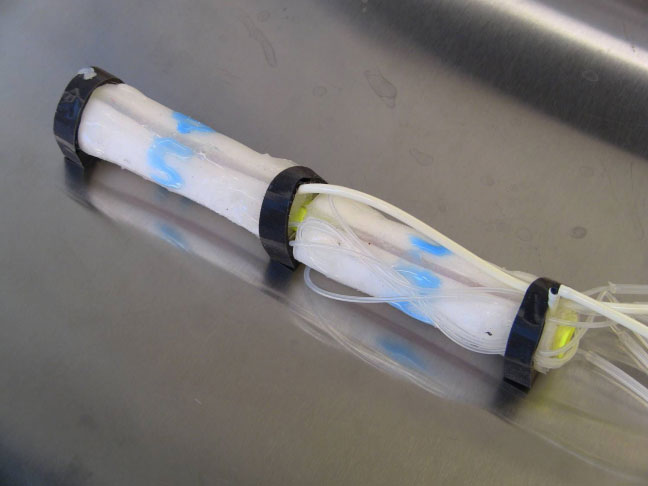
\includegraphics[width=\linewidth]{figures/jamming/jmu-worm}
    \caption[Jamming Modulated Unimorph by \citet{steltz2010jamming}.]
    {Jamming Modulated Unimorph \citep{steltz2010jamming}.}
    \label{fig:ch:jamming:jmu}
  \end{minipage}
\end{figure}

\subsubsection{Human-computer Interaction}
\label{ch:jamming:related-work:hci}
Jamming has also been explored in the area of HCI though to a limited extent.
Most of the examples here are very recent contributions (2012) but they do show promising applications.

\paragraph{Dynamically changeable physically buttons (\citeyear{harrison2009providing})} 
\label{ch:jamming:related-work:hci:dynbuttons}
This first example is actually not based on jamming but on some of the same principles, where pneumatic actuation is used to enable deformations on a latex surface.
The project presents a visual display which contains deformable areas able to create physical buttons.
An acrylic backing layer with cut-out areas for the shapes and positions of the buttons are placed under an upper latex surface.
With pneumatic control it is possible to dynamically make physical buttons appear at the cut-out areas as either convex, concave, or flat forms, see figure~\ref{fig:ch:jamming:concepts:harrisonhudson}.
Though button states can be modified they are still in a very static configuration due to the cut-out areas which cannot be changed.

\begin{figure}[h]
  \centering
  \begin{minipage}[b]{.8\textwidth}
    \centering
    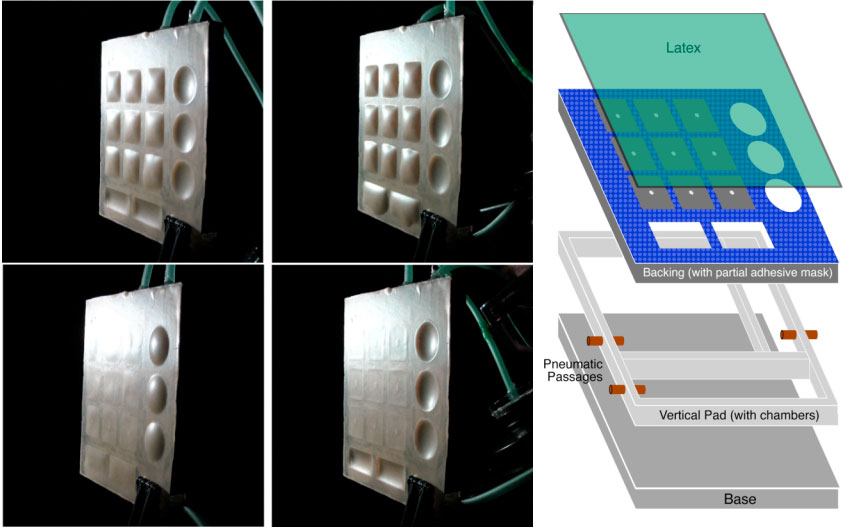
\includegraphics[width=.7\linewidth]{figures/jamming/harrisonhudson}
    \caption{A tactile display in various interface states. All buttons are statically positioned \citep{harrison2009providing}.}
    \label{fig:ch:jamming:concepts:harrisonhudson}
  \end{minipage}
\end{figure}

\paragraph{The HoverMesh (\citeyear{mazzone2004hovermesh})}
\label{ch:jamming:related-work:hci:hovermesh}
\citet{mazzone2004hovermesh} did some early work on creating a deformable structure with the jamming technique. 
The HoverMesh prototype is a cell-based jamming system consisting of 3x3 grid, see figure~\ref{fig:ch:jamming:hovermesh}.
The grid is mounted on top of a cubicle which can be inflated and deflated and together with the grid it creates deformations of the surface structure.
The HoverMesh prototype is not fully implemented according to the ideas presented.
It consists only of the grid structure on top of the cubicle and does not exhibit input capabilities through vision-based techniques and haptic feedback output as intended. 

\paragraph{ClaytricSurface (\citeyear{matoba2012claytricsurface})}
\label{ch:jamming:related-work:hci:claytric}
\citet{matoba2012claytricsurface} created a flexible tabletop surface, ClaytricSurface, which serves as a sculptable display medium (see figure~\ref{fig:ch:jamming:claytric-surface}). 
The surface can be directly manipulated by hand and the stiffness can be controlled in real time by a GUI slider.
Input is detected by a depth camera from above the tabletop.
The exemplified application of ClaytricSurface is a painting application projected onto the surface from above and a user can use direct touch on the surface to draw. 
ClaytricSurface uses the basic jamming approach and demonstrates the use of a rather large jammable surface area with direct manipulation abilities.

\begin{figure}
  \centering
  \begin{minipage}[t]{.44\textwidth}
    \centering
    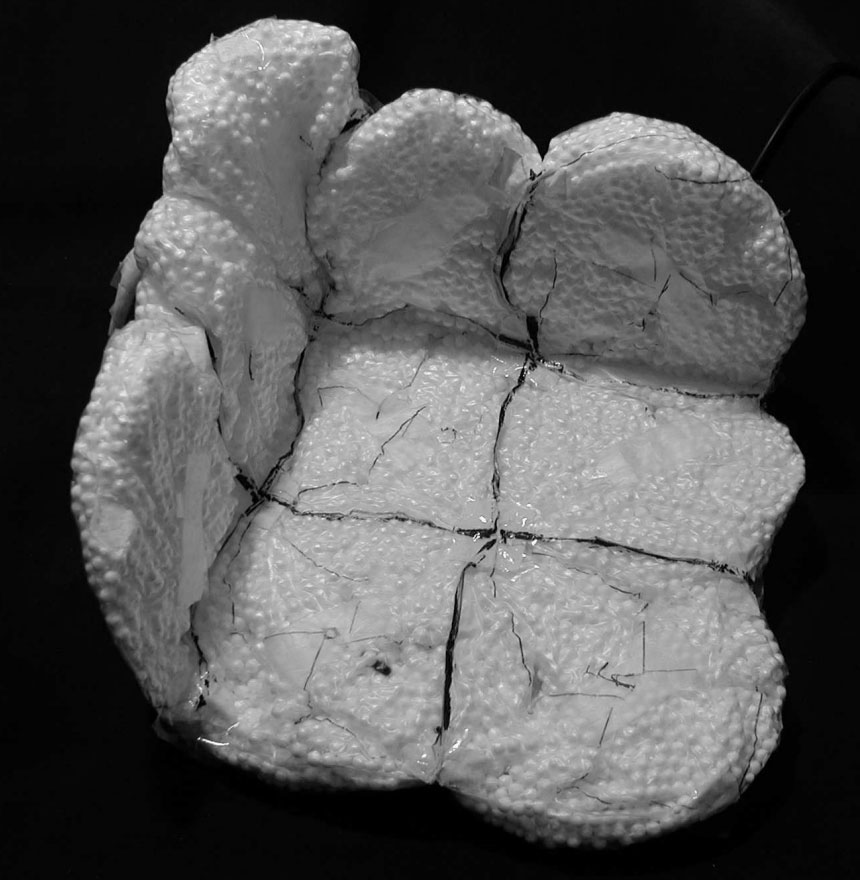
\includegraphics[width=\linewidth]{figures/jamming/hovermesh}
    \caption[The HoverMesh by \citet{mazzone2004hovermesh}.]
    {The HoverMesh \citep{mazzone2004hovermesh}.}
    \label{fig:ch:jamming:hovermesh}
  \end{minipage}%
  \hspace{0.02\textwidth}
  \begin{minipage}[t]{.44\textwidth}
    \centering
    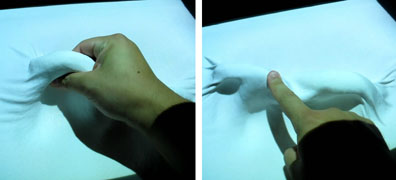
\includegraphics[width=\linewidth]{figures/jamming/claytric-surface}
    \caption[Claytric Surface by \citet{matoba2012claytricsurface}.]
    {Claytric Surface \citep{matoba2012claytricsurface}.}
    \label{fig:ch:jamming:claytric-surface}
  \end{minipage}
\end{figure}

\paragraph{Jamming User Interfaces (\citeyear{follmer2012jamming})}
\label{ch:jamming:related-work:hci:jui} 
\citet{follmer2012jamming} have probably made the biggest contribution yet to the use of jamming in HCI. 
The authors coin the approach \textit{Jamming User Interfaces} and position it in the area of malleable and organic user interfaces. 
They make several contributions to the field by exploring jamming interfaces for haptic feedback, for malleable tabletops and for mobile devices (see figure~\ref{fig:ch:jamming:jui-collection}). 
They also investigate how sensing techniques like capacitive and optical sensing, can broaden the applicability of jamming in HCI. 

\citet{follmer2012jamming} also present a hydraulic jamming system that is fast and silent and which allows for semi-transparent jamming volumes. 
This requires transparent particles, such as glass-beads, and a transparent fluid that matches the refractive index of the particles so that light refraction is reduced, see figure~\ref{fig:ch:jamming:jui:refractive}. 

\begin{figure}[h]
  \centering
  \begin{minipage}[b]{.7\textwidth}
    \centering
    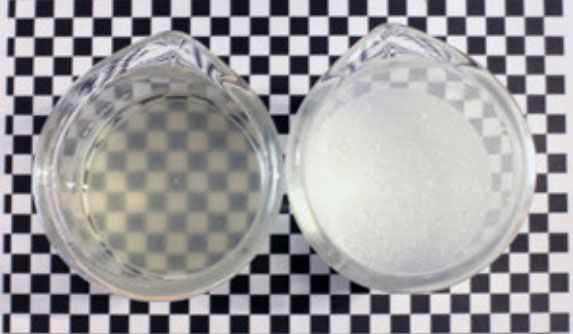
\includegraphics[width=.5\linewidth]{figures/jamming/refractive-index}
     \caption{Transparency obtained by matching the refractive index of the glass-bead particles \citep{follmer2012jamming}}.
    \label{fig:ch:jamming:jui:refractive}
  \end{minipage}
\end{figure}

In the following we will give a brief overview of the four prototypes implemented and described by \citet{follmer2012jamming}.

\subparagraph{Tunable Clay} is a malleable tabletop for direct 3D modelling (see figure~\ref{fig:ch:jamming:jui-clay}).
It resembles ClaytricSurface \citep{matoba2012claytricsurface} mentioned earlier with its clay-like surface that can easily be deformed (basic jamming approach).
Tunable Clay uses the hydraulic jamming system mentioned above with index-matched particles and fluid.
This allows for a more sophisticated depth sensing approach than the one used with ClaytricSurface.
Optical shape sensing and graphic projection is integrated underneath the jamming volume.
The shape, captured in real-time, is shown as a virtual 3D model on both an external display and on the jamming volume itself projected from underneath the surface.

\subparagraph{Transparent Haptic Lens} is a small tangible puck to be used as a haptic information channel on a tabletop display (basic jamming approach), see figure~\ref{fig:ch:jamming:jui-lens}.
It has a transparent lens in the center which is a transparent hydraulic jamming volume that can change its stiffness according to the texture beneath it.
By pressing ones finger into the lens the user can get a haptic sensation through stiffness reflecting the underlying texture of the image directly underneath. 

\subparagraph{Behind-the-Tablet Jamming} is a tablet computer which has a pneumatic jamming volume mounted on the backside (basic jamming approach), see figure~\ref{fig:ch:jamming:jui-tablet}.
The system senses malleable input with capacitive shape sensing.
The scenarios envisioned are for navigating content (e.g. scrolling and zooming) on the tablet display through malleable interaction on the backside. 
The system can communicate that some limit is reached with haptic feedback, 
e.g. by stiffening the jamming volume.

\subparagraph{ShapePhone} is a generic mobile device that can be shaped and locked into different forms (basic jamming approach).
The device has no technology inside, except for the jamming system, and it merely serves as demonstration of how its affordances change when it is sculpted into forms resembling e.g. a phone, a remote control or a watch (see figure~\ref{fig:ch:jamming:jui-phone}).
Ideas are presented for integrating various sensing techniques such as capacitive shape sensing and touch sensing to derive contextual information.

\begin{figure}
        \centering
        \begin{subfigure}[b]{0.44\textwidth}
                \centering
                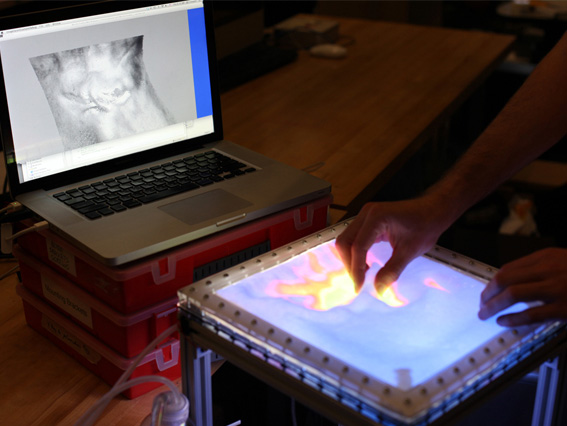
\includegraphics[width=\textwidth]{figures/jamming/jui_tunable-clay}
                \caption{Tuneable Clay}
                \label{fig:ch:jamming:jui-clay}
        \end{subfigure}
        \hspace{0.02\textwidth}
        \begin{subfigure}[b]{0.44\textwidth}
                \centering
                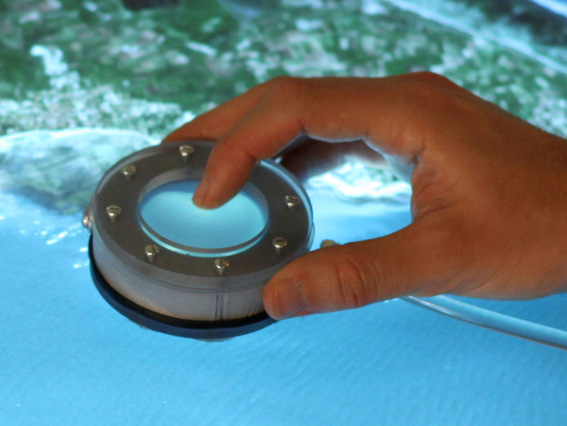
\includegraphics[width=\textwidth]{figures/jamming/jui_haptic-lens}
                \caption{Transparent Haptic Lens}
                \label{fig:ch:jamming:jui-lens}
        \end{subfigure}

        \begin{subfigure}[b]{0.44\textwidth}
                \centering
                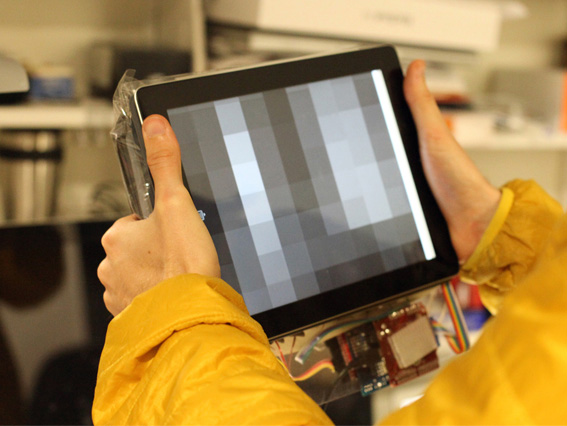
\includegraphics[width=\textwidth]{figures/jamming/jui_behind-the-tablet}
                \caption{Behind-the-Tablet Jamming}
                \label{fig:ch:jamming:jui-tablet}
        \end{subfigure}
        \hspace{0.02\textwidth}
        \begin{subfigure}[b]{0.44\textwidth}
                \centering
                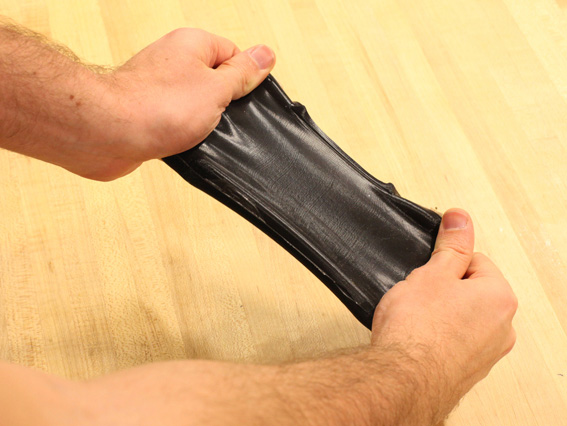
\includegraphics[width=\textwidth]{figures/jamming/jui_shapephone}
                \caption{ShapePhone}
                \label{fig:ch:jamming:jui-phone}
        \end{subfigure}
        \caption{Jamming User Interfaces by \citet{follmer2012jamming}.}
        \label{fig:ch:jamming:jui-collection}
\end{figure}

\subsection{Summary of related work}

In the previous sections we have given an introduction to the mechanics of jamming and an overview of different research applications of jamming.
These applications show two primary approaches to jamming.
The first one is the basic approach where a single volume containing particles can be jammed by applying a vacuum inside (see figure~\ref{fig:ch:jamming:approaches:basic}).
Applications of the basic approach are for example the \emph{Claytric Surface} and \emph{ShapePhone}.
The other is the more complicated cell-based approach where each cell is an independent jammable volume working in the same manner as the basic approach.
As the cells exist on the perimeter of the volume some other compound must constitute the body of the volume and stabilise the form.
In \emph{The HoverMesh} this was air inside a cubicle and in \emph{JSEL} it was fluid (see figure~\ref{fig:ch:jamming:approaches:cell}).

The related work demonstrate different potentials for the use of jamming through implementations based on mechanics, direct manipulation, shape-change, and as a feedback channel.
In table \ref{ch:jamming:table:applications_overview} we have summarises and categorises the mentioned applications according to their characteristics.
In the next section we will move on to our own concepts that support the notion of ad hoc interfaces.

\begin{landscape}
  \thispagestyle{empty}
  \centering 
  \captionof{table}{An overview and categorisation of related jamming work}
  \label{ch:jamming:table:applications_overview} 
  \begin{tabularx}{\linewidth}{|l|c|c|c|c|c|X|}
    \hline
    Project                 & Input                         & Output                        & Type      & Particles   & Approach  & Summary \\ \hline
    \hline
    Robotic gripper         & \cellcolor{FalseColor}\xmark  & \cellcolor{TrueColor}\cmark   & pneumatic & coffee      & basic     & A universal robotic gripper \\ \hline
    Jamming Skin Enabled Locomotion & \cellcolor{FalseColor}\xmark  & \cellcolor{TrueColor}\cmark   & pneumatic & glass beads     & cell-based& A soft moving robot \\ \hline
    Jamming Modulated Unimorph & \cellcolor{FalseColor}\xmark  & \cellcolor{TrueColor}\cmark   & pneumatic & glass beads          & cell-based& A worm-like robot \\ \hline
    \hline
    The HoverMesh           & \cellcolor{FalseColor}\xmark  & \cellcolor{TrueColor}\cmark   & pneumatic & polystyrene & cell-based& A cell-based deformable surface structure . \\ \hline    
    ClaytricSurface         & \cellcolor{TrueColor}\cmark   & \cellcolor{FalseColor}\xmark  & pneumatic & polystyrene & basic     & A flexible tabletop surface which serves as a sculptable display medium. \\ \hline
    Tunable Clay            & \cellcolor{TrueColor}\cmark   & \cellcolor{FalseColor}\xmark  & hydraulic & glass beads & basic     & A malleable tabletop for direct 3D modelling. \\ \hline
    Transparent Haptic Lens & \cellcolor{FalseColor}\xmark  & \cellcolor{TrueColor}\cmark   & hydraulic & glass beads & basic     & A small tangible puck to be used as a haptic information channel on a tabletop display. \\ \hline
    Behind-the-Tablet       & \cellcolor{TrueColor}\cmark   & \cellcolor{TrueColor}\cmark   & pneumatic & ?           & basic     & A tablet with a interactive jamming volume on the back. \\ \hline
    ShapePhone              & \cellcolor{TrueColor}\cmark   & \cellcolor{FalseColor}\xmark  & pneumatic & coffee      & basic     & a generic mobile device that can be shaped and locked into different forms. \\
    \hline
  \end{tabularx}

  \begin{flushleft}
  This table is an overview and categorisation of the prototypes presented in the papers covered in this section. It should be mentioned that in categorising \textit{input} and \textit{output} features we are only considering whether input or output is enabled using the jamming technique. For example, \textit{Tunable Clay} does have output in the form a image projection but it does not utilise the jamming technique.
  \end{flushleft}

\end{landscape}


\section{Exploring jamming concepts}
\label{ch:jamming:concepts} 
%!TEX root = ../thesis.tex
This section will focus on describing and discussing a selection of concepts for ad hoc interfaces based on the jamming technique.
As mentioned in the beginning of this chapter we were not successful at implementing a working jamming system where we could effectively control air/liquid flow.
Therefore we concentrate on conceptual prototypes which we envisioned before taking the decision to move in other directions.
Each of these concepts have different focal points.
The first one, \emph{\nameref{ch:jamming:concepts:dynamic_input}}, strives to achieve on-demand standard interfaces for input control.
The second, \emph{\nameref{ch:jamming:concepts:playful_blobs}}, seeks to draw on known interaction metaphors from the digital world and expose them to physical objects.
The third, \emph{\nameref{ch:jamming:concepts:improvised_furniture}}, scales up the dimensions and focuses on a living environment with highly configurable components.

\subsection{Dynamic input controls} 
\label{ch:jamming:concepts:dynamic_input}

This concept was our starting point for our first endeavours with jamming.

The concept resembles the work of \citet{harrison2009providing} mentioned in the related work section and our intentions were also to create physical input controls with the dynamic qualities of the digital counterpart.
But we were of the opinion that by using the jamming technique we could overcome some of the constraints of their approach and offer even more flexibility.
The limitations of the approach taken by \citet{harrison2009providing} were primarily the reliance on a backing layer where cut-out areas determined the position and shape of the buttons.
They were able to show a button either in convex or concave form or not at all, but the buttons were locked in their positions and the shapes were also not modifiable.

Instead, we propose using the jamming technique with a cell-based approach.
Individual cells can be used to create deformations on different areas of the surface and the composition of multiple cells makes it possible to make forms of heterogeneous shapes emerge anywhere on the plane, see figure \ref{fig:ch:jamming:concepts:button-cells}.
The idea of composition is quite similar to the that of computer graphics where polygons are used to compose images that are appear three-dimensional.
In this way, not only can we make input controls appear and disappear, we can also change the shape and position of them for an even more dynamic interface.

As a simple example we made mocked up a prototype to demonstrate simple shapes by jamming.
Due to our issues with a jamming, this was again a setup with a vacuum cleaner, plastic bag as the membrane, and ground coffee as the particles, see figure \ref{fig:ch:jamming:concepts:inputs-prototype}.

\begin{figure}[h]
  \centering
  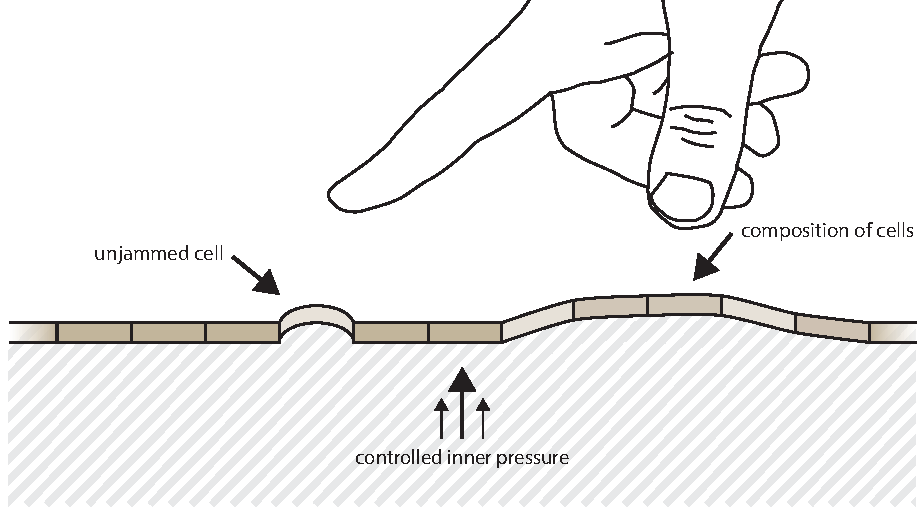
\includegraphics[width=.9\textwidth]{figures/jamming/concepts/jamming-inputs-concept.pdf}
  \caption{A cross-sectional view of a cell-based button and a composition multiple cells with different pressures for complex forms.}
  \label{fig:ch:jamming:concepts:button-cells}
\end{figure}

%We conceptualize on household appliances such as radios, clock alarms, house alarms heating, ventilation and air conditioning (HVAC), \todo{etc}.
%In general physical products with standard input controls such as buttons, knobs, switches and sliders.

\begin{figure}[h]
\centering
\begin{subfigure}[t]{.44\textwidth}
  \centering
  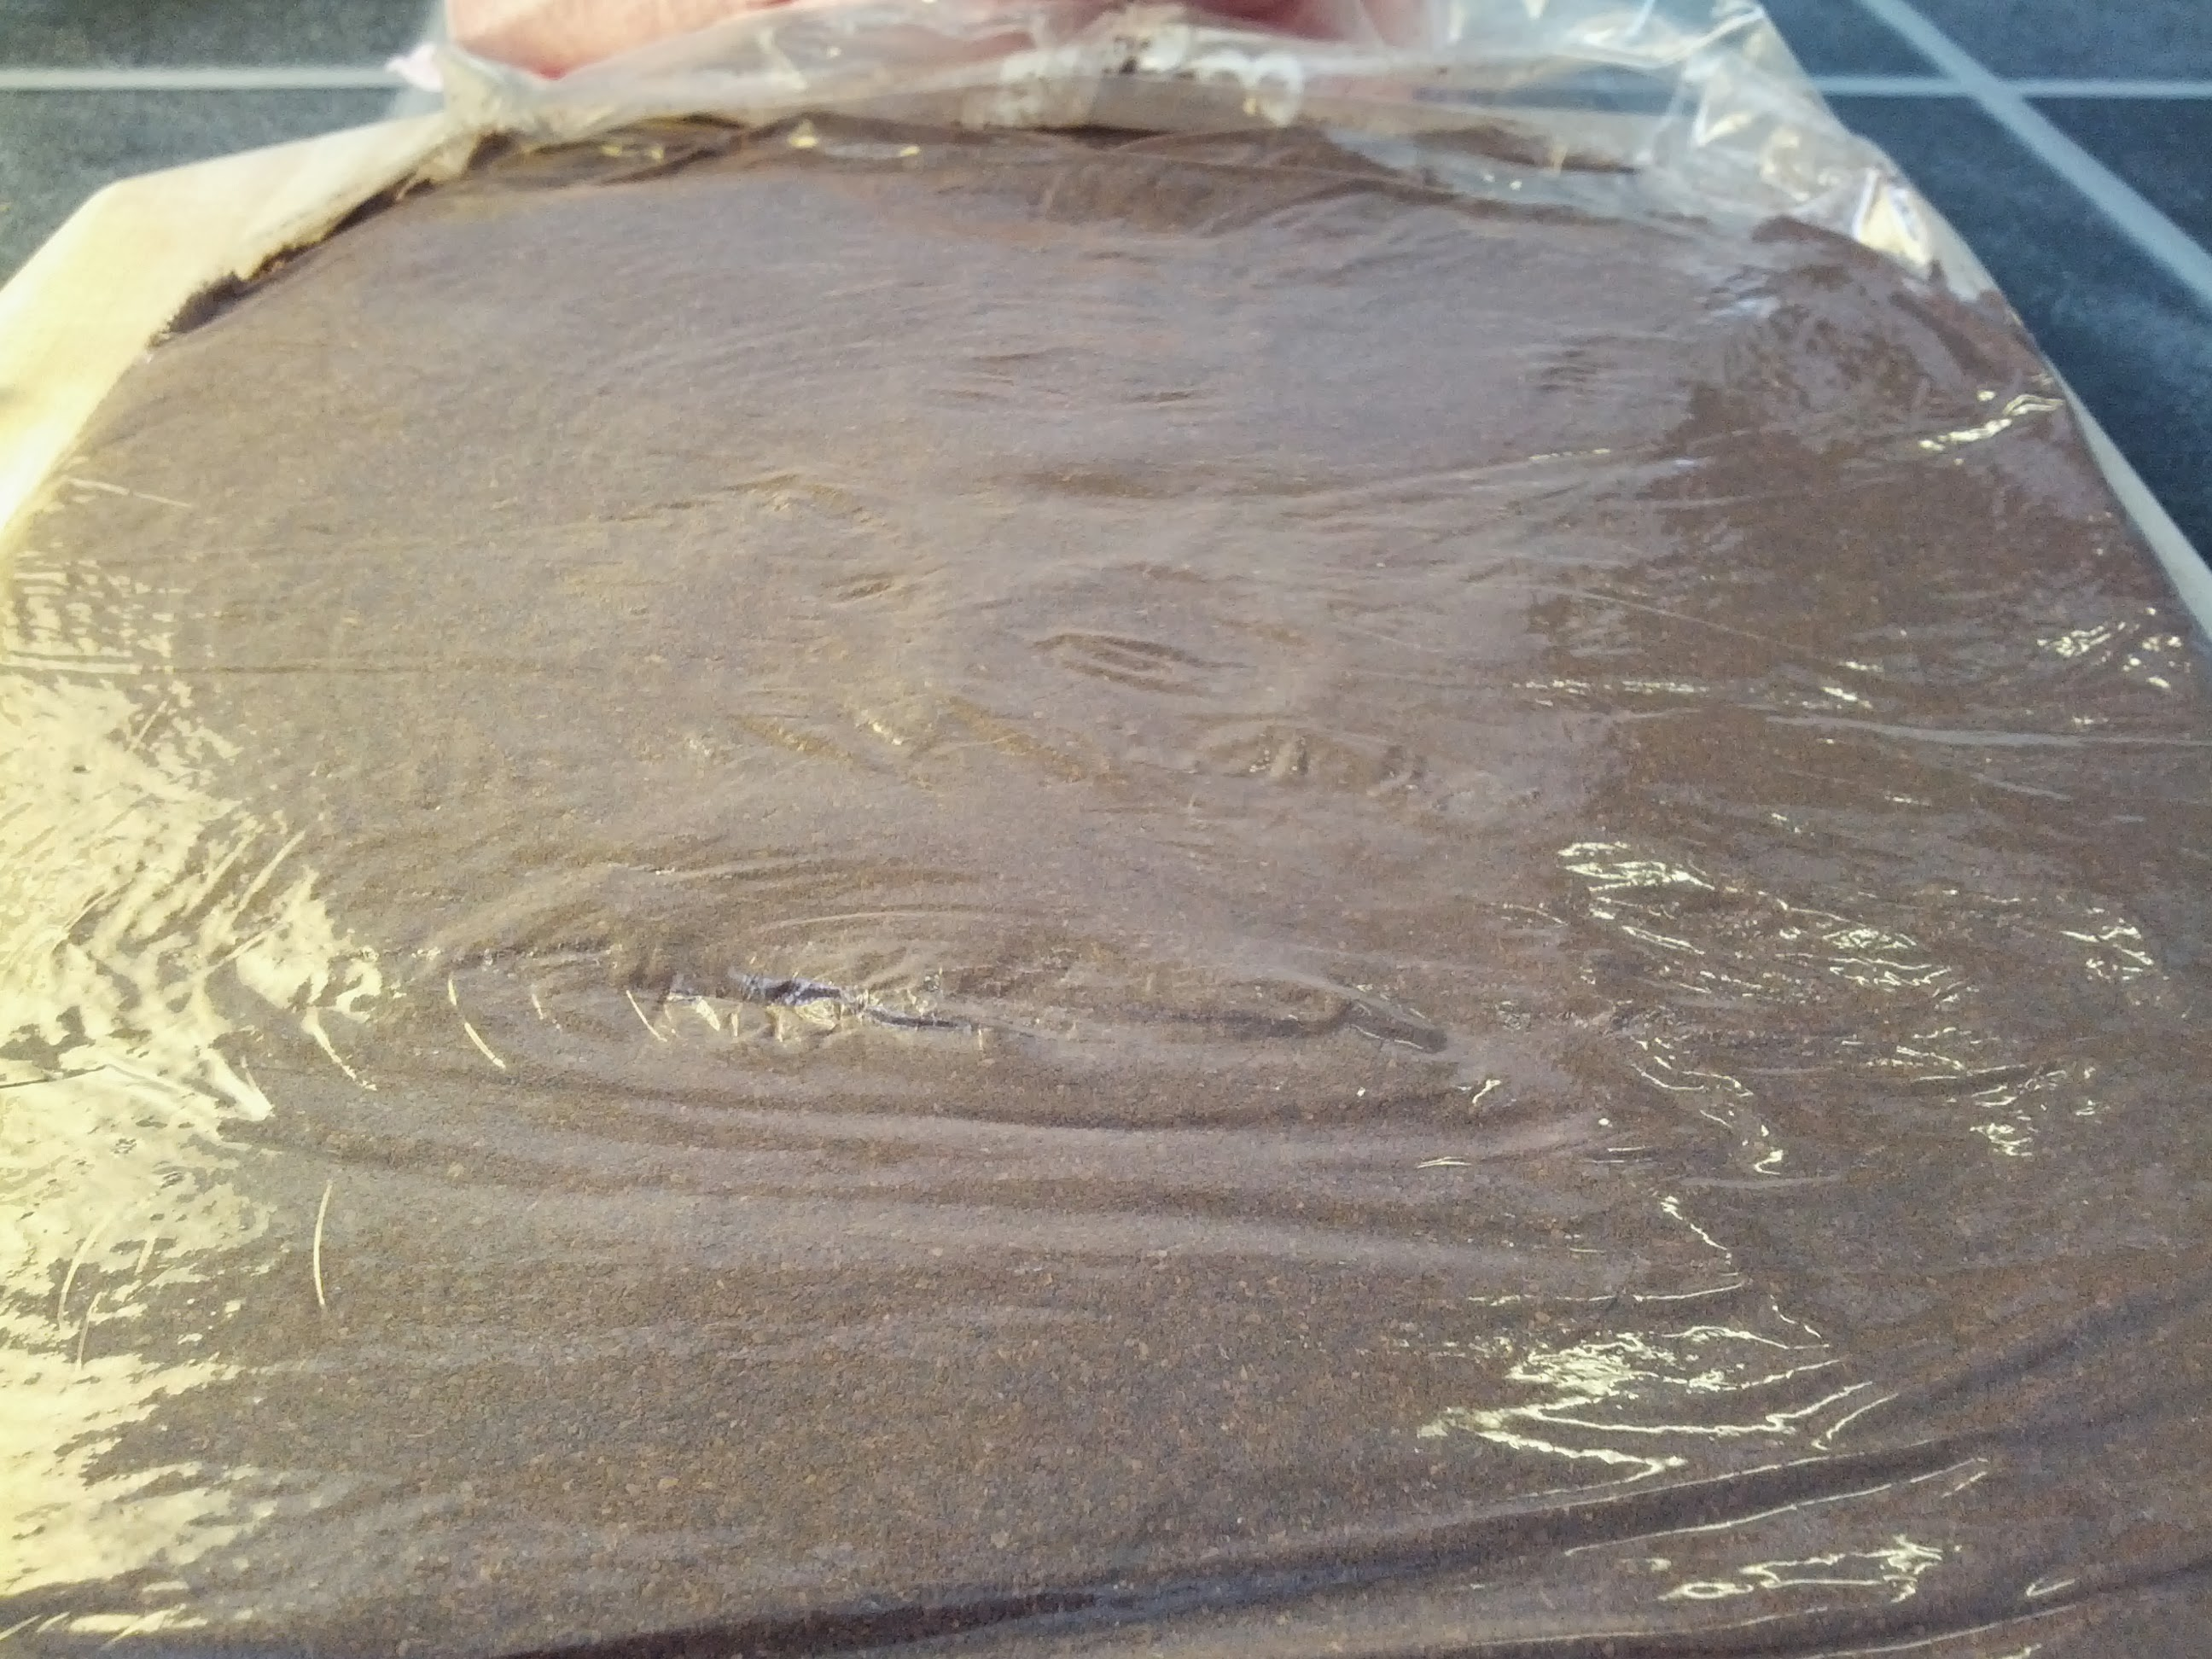
\includegraphics[width=\linewidth]{figures/jamming/concepts/inputs/jamming-inputs-flat}
    \caption{A flat surface with the absence of any input controls.}
\end{subfigure}%
\hspace{0.02\textwidth}
\begin{subfigure}[t]{.44\textwidth}
  \centering
  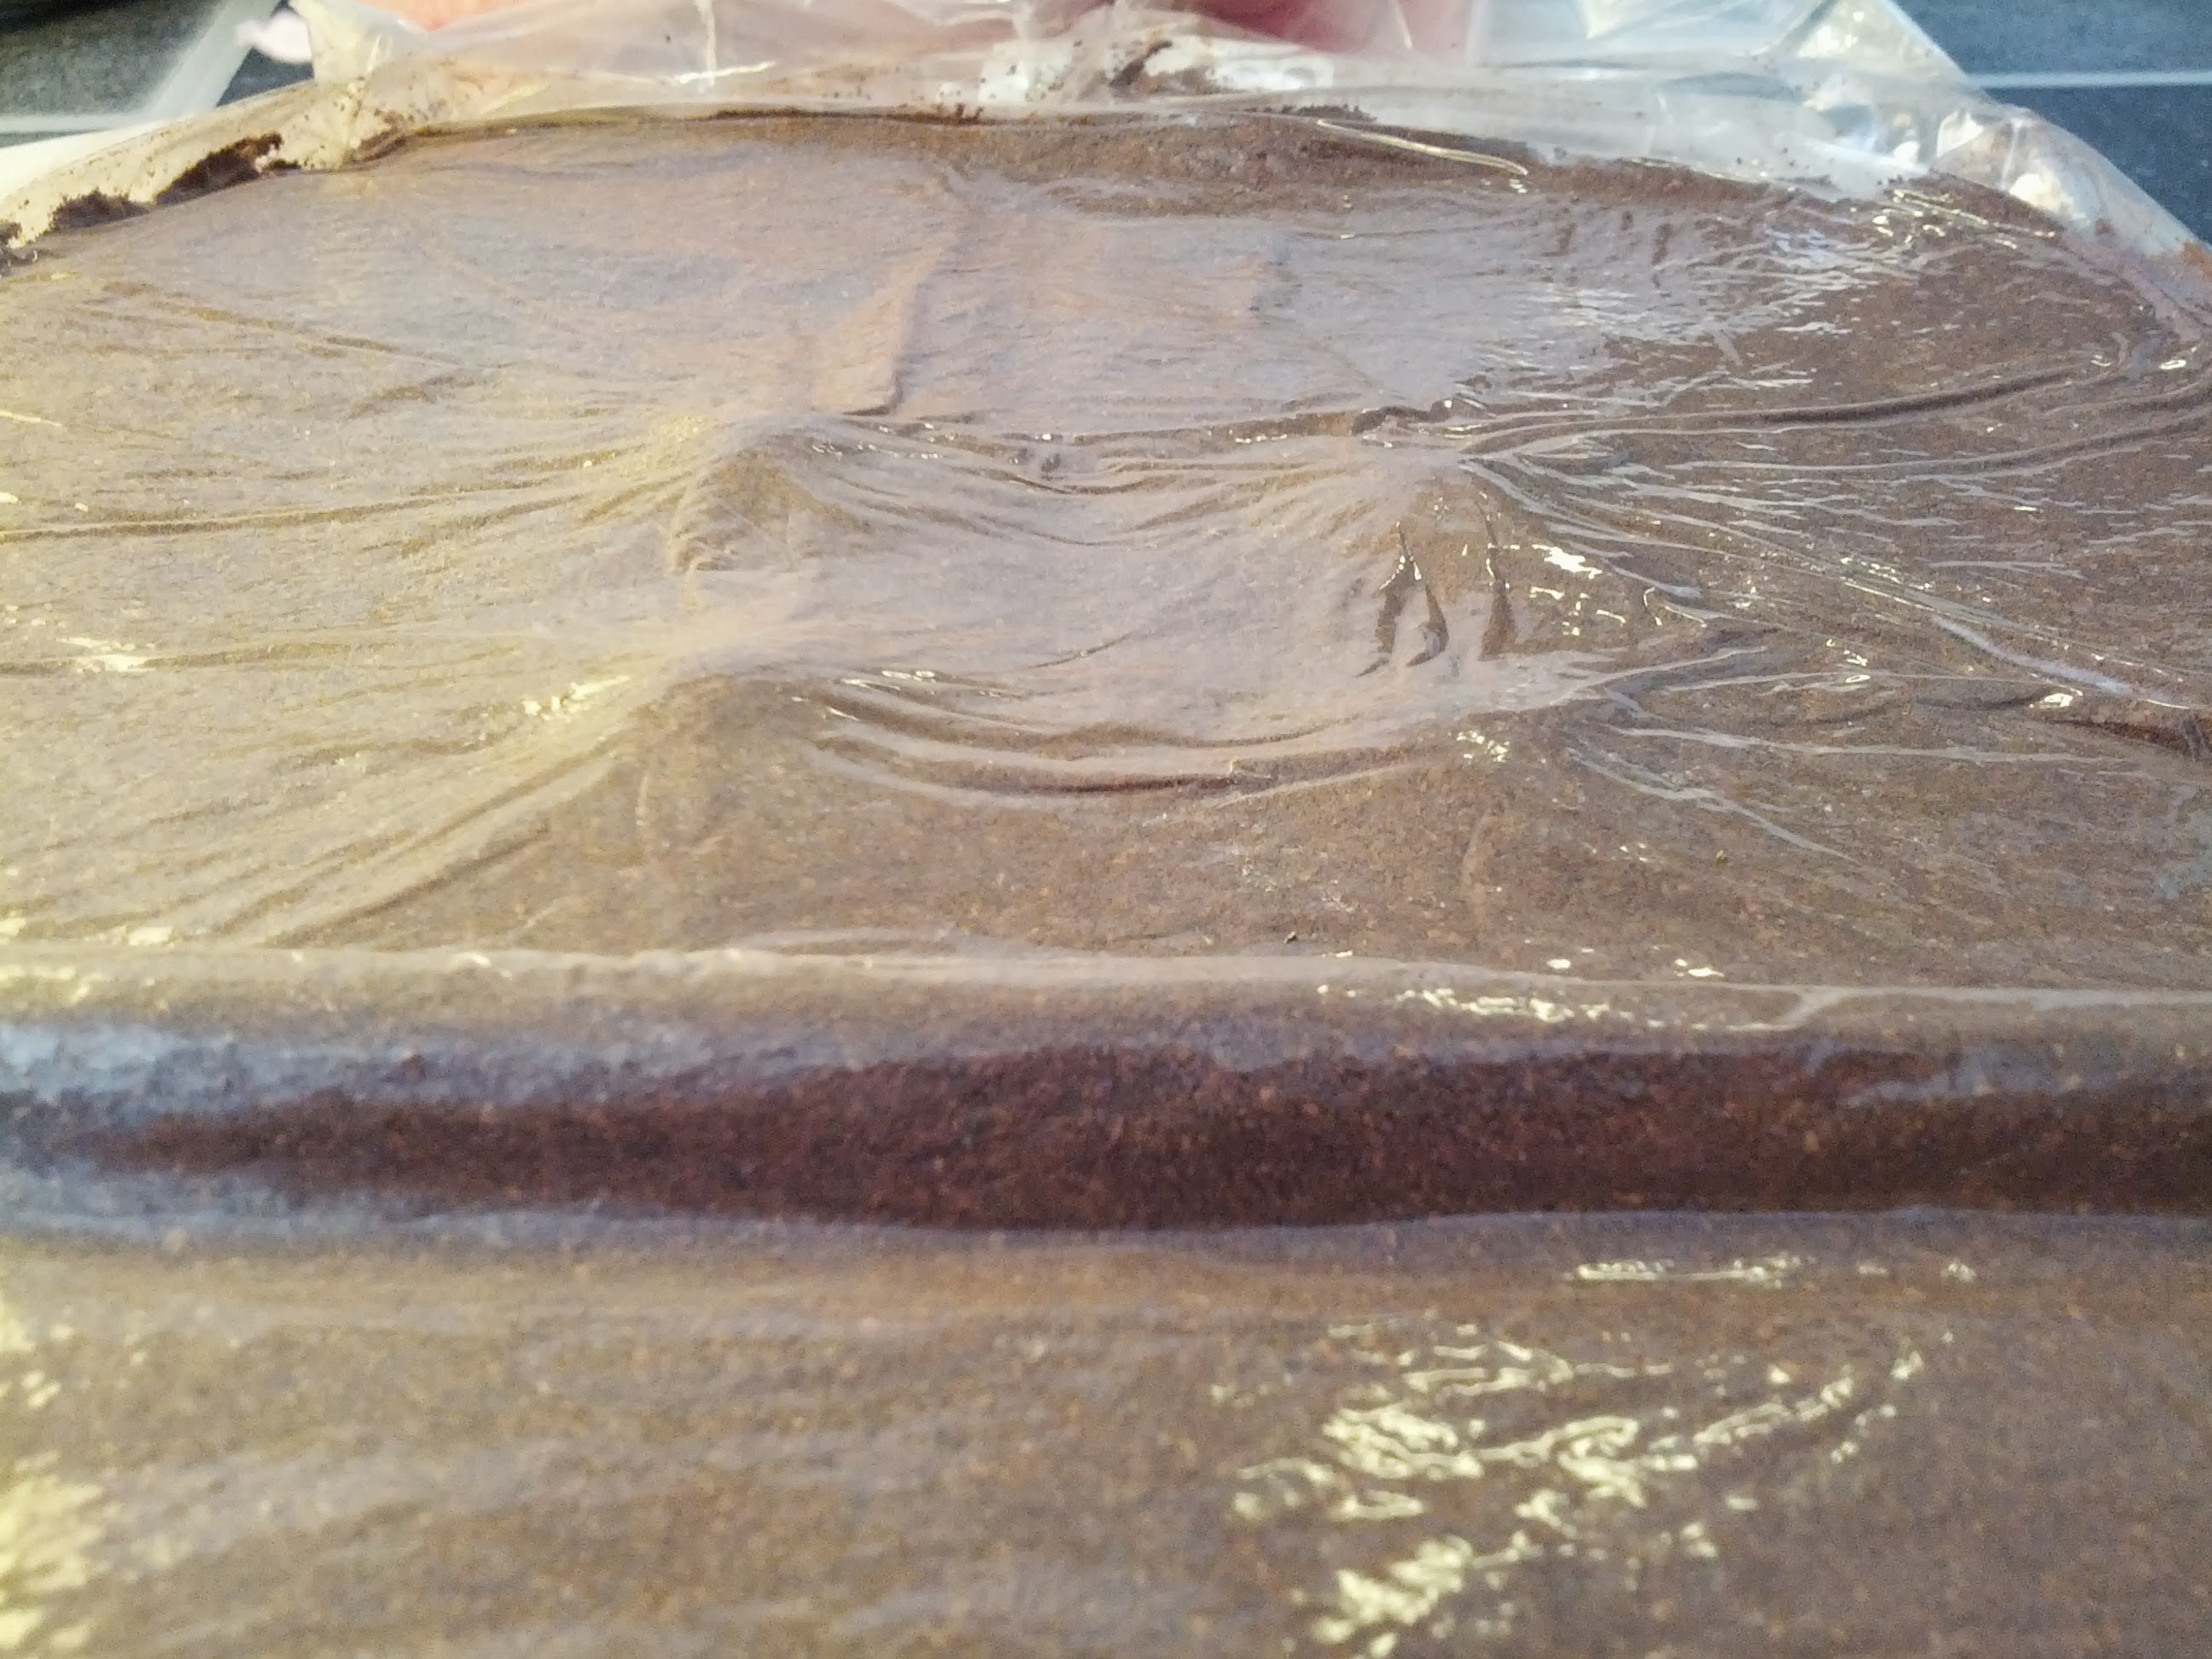
\includegraphics[width=\linewidth]{figures/jamming/concepts/inputs/jamming-inputs-buttons}
  \caption{Four buttons have emerged and an elongated input control for e.g. sliding or grabbing and pulling.}
\end{subfigure}
\caption{A primitive exploratory prototype with basic jamming of a single volume. Ground coffee is enclosed withing a transparent plastic bag. Wrinkles occur due to the plastic bag not being very flexible.}
\label{fig:ch:jamming:concepts:inputs-prototype}
\end{figure}

\subsection{Playful blobs}
\label{ch:jamming:concepts:playful_blobs}

The focal point of this next concept is on bringing input and output into the same object.
As can be seen in table~\ref{ch:jamming:table:applications_overview} on page~\pageref{ch:jamming:table:applications_overview} only one of the listed projects from the related work section, \nameref{fig:ch:jamming:jui-tablet}, has both input and output in same object.
Therefore we see an unexplored area of jamming potentials which we would like to address in the this next concept.

We envision a toy concept for children which we call \nameref{ch:jamming:concepts:playful_blobs}.
The blobs are tangible clay-like objects meant to be moulded into creative forms.
Each blob makes a selection of commands available otherwise known from digital interface metaphors, such as \emph{save, open, undo, delete, copy, and paste} which can actuate the blob in different ways.
These commands give a physical blob a notion of form memory where state is kept over time.
If needed previously saved forms can be recalled and further work on the form can done.
More specifically each command means (see also figure~\ref{fig:ch:jamming:concepts:blobs:states}):
\begin{itemize}
	\item{\emph{Save}: The current form of a blob is saved in memory for later retrieval.}
	\item{\emph{Open}: A previously saved form can be recalled and the blob actuates itself into the saved state.}
	\item{\emph{Undo}: Negate the latest moulding of the blob.}
	\item{\emph{Copy}: Make a copy of the state of a specific blob. The copied state could be saved in a blob or in an external object.}
	\item{\emph{Paste}: Set the state of a blob to that of which has been copied.} 
	\item{\emph{Delete}: Reset a blob so that all state is forgotten.} 
\end{itemize}

\begin{figure}[h]
  \centering
  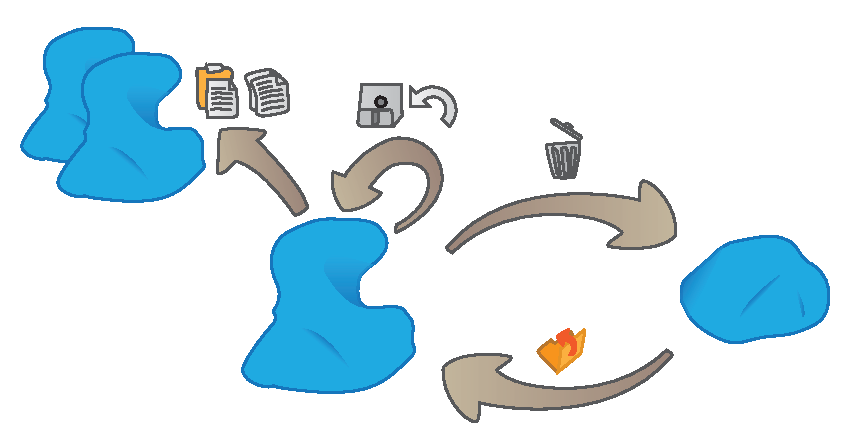
\includegraphics[width=.9\textwidth]{figures/jamming/concepts/blobs/state-transitions.pdf}
  \caption{A visualisation of the different commands and the associated state transititons.}
  \label{fig:ch:jamming:concepts:blobs:states}
\end{figure}

The commands are made possible via a cell-based jamming structure and the amount of detail a moulded blob can have is dictated by the resolution of the jamming cells.
As mentioned earlier this jamming approach makes it possible to separately control the stiffness of each cell.
So, for example, the \emph{save} command is done by storing a map of the current pressure states of each cell.
A subsequent \emph{open} or \emph{paste} command would set the correct pressure values of the cells and thereby restore the \emph{saved} or \emph{copied} physical form.
Lastly, a \emph{delete} command would release all negative pressure in cells and thereby collapse the form.
A simple prototype is shown figure~\ref{fig:ch:jamming:concepts:blobs:gloves} made with the basic jamming approach.
The actuation process would have to be done in a correct sequence in order for specific curvatures to become possible, which presumably could be done by computation.

\begin{figure}[h]
  \centering
  \begin{subfigure}[t]{.28\textwidth}
    \centering
    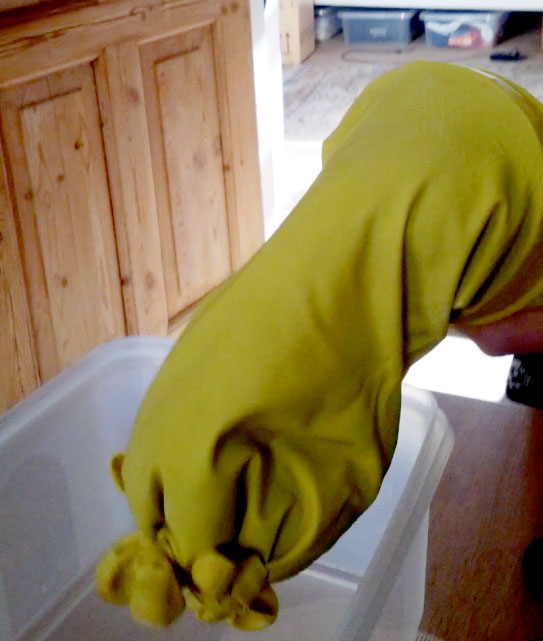
\includegraphics[width=\linewidth]{figures/jamming/concepts/blobs/glove-1.jpg}
    \captionof{figure}{The blob in collapsed state, i.e. no pressure is upheld.}
    \label{fig:ch:jamming:concepts:blobs:g1}
  \end{subfigure}%
  \hspace{0.03\textwidth}
  \begin{subfigure}[t]{.28\textwidth}
    \centering
    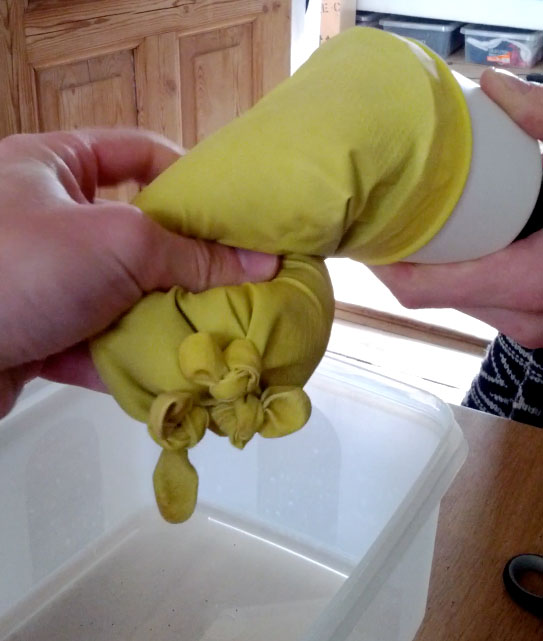
\includegraphics[width=\linewidth]{figures/jamming/concepts/blobs/glove-2}
    \captionof{figure}{The blob being molded into a custom shape.}
    \label{fig:ch:jamming:concepts:blobs:g2}
  \end{subfigure}
  \hspace{0.03\textwidth}
  \begin{subfigure}[t]{.28\textwidth}
    \centering
    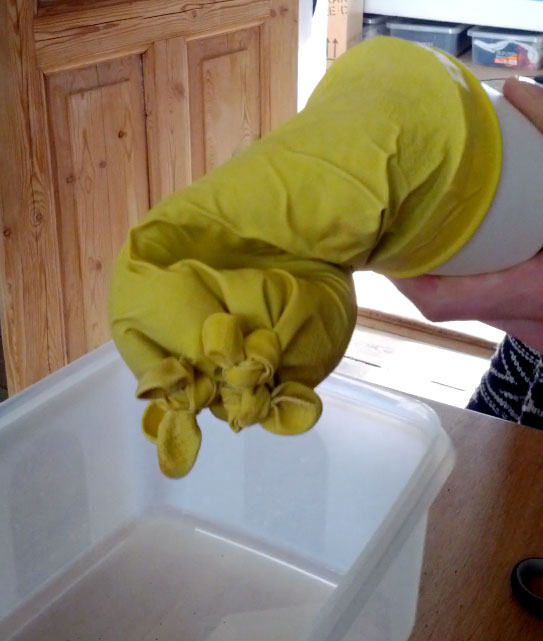
\includegraphics[width=\linewidth]{figures/jamming/concepts/blobs/glove-3}
    \captionof{figure}{The shape of the blob is maintained.} 
    \label{fig:ch:jamming:concepts:blobs:g3}
  \end{subfigure}
  \caption{An exploratory prototype of playful blobs. Created with a rubber latex glove, ground coffee, and a vacuum cleaner. For a video of the above steps see appendix~\ref{app:videos:jamming} which also shows the rigidity of the shape when jammed.}
  \label{fig:ch:jamming:concepts:blobs:gloves}
\end{figure}

We envision that the blobs can be used in a clay-like manner for kids to explore moulding of material into various forms and where particular interesting forms can be saved, duplicated and so on.
Furthermore, we also envision that these blobs could be used as the foundation for a new kind of dynamic building block for construction toys.
A concept that takes products such as Lego\footnote{http://www.lego.com/} a step further by having building blocks that are deformable and can be locked into any shape by the use of jamming.
This allows for block shapes that are no more limited to the supply of the production company but which allow for custom moulded blocks that are adapted to the needs of the user.

Applying these digital features to the physical blobs exhibits ad hoc qualities where the shape itself forms the interface and where shapes can be created on an ad hoc basis.
When a particular shape is no longer needed it can disappear again by remoulding it or letting it collapse (jamming-wise).

\subsection{Improvised furniture}
\label{ch:jamming:concepts:improvised_furniture}

This concept is based on replacing static components of the home with dynamic jamming enabled substitutes.
In its most extreme case with a large scale deployment it may be a little far fetched but an intriguing thought experiment and maybe not that unrealistic in a more futuristic scenario.
It underpins the idea of a configurable home where otherwise static and massive components such as walls and furniture allow for deformations.
For example, pushing in part of a wall to make room for a plant or even an entire shelf.
Or, deforming the floor to improvise an extra seat for a guest.
Or, adjusting the armrest or back of the sofa for a more comfortable position.

These examples correlate with what we touched upon in \autoref{ch:domain} about Steward Brands understanding of changes in a building;
Pulling down a given layer of change to a lower layer to create a more dynamic and adaptable environment.
The concept of improvised furniture would then be \emph{Space Plan} elements that are exposed to the layer of \emph{Stuff}. 
Figure~\ref{fig:ch:jamming:concepts:impro} illustrates deformation of walls for improvised furniture.

With this reconfigurability done by hand the components will naturally end up having an organic appearance with curvatures and very few straight lines and edges.

Using jamming in a large scale deployment where strength and bearing capacity is a requirement does come with quite a few constraints regarding materials.
The container of the particles must be strong enough to handle the exposed level of stress and strain while still being flexible enough to allow for surface deformations.

\begin{figure}[h]
  \centering
  \begin{subfigure}[t]{.44\textwidth}
    \centering
    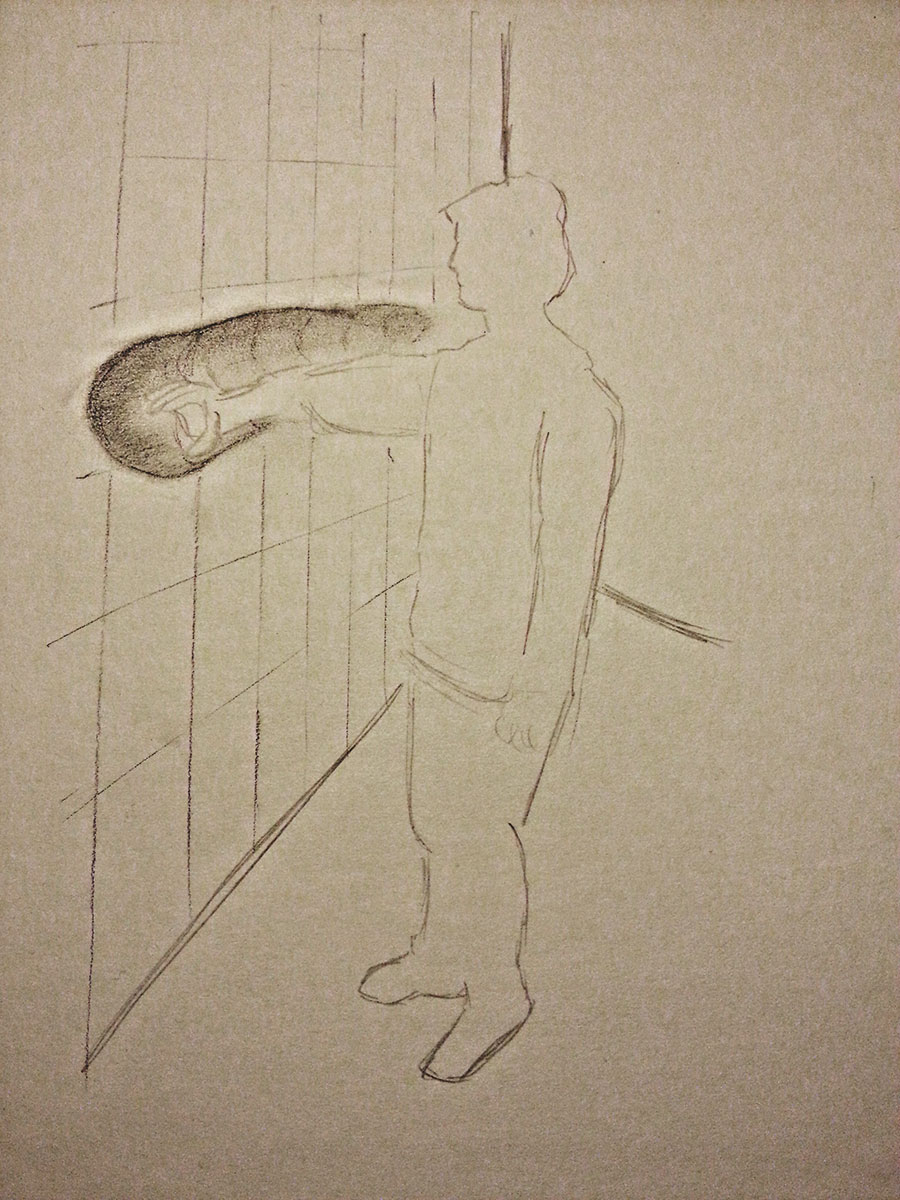
\includegraphics[width=\linewidth]{figures/jamming/concepts/impro/carve}
  \end{subfigure}%
  \hspace{0.02\textwidth}
  \begin{subfigure}[t]{.44\textwidth}
    \centering
    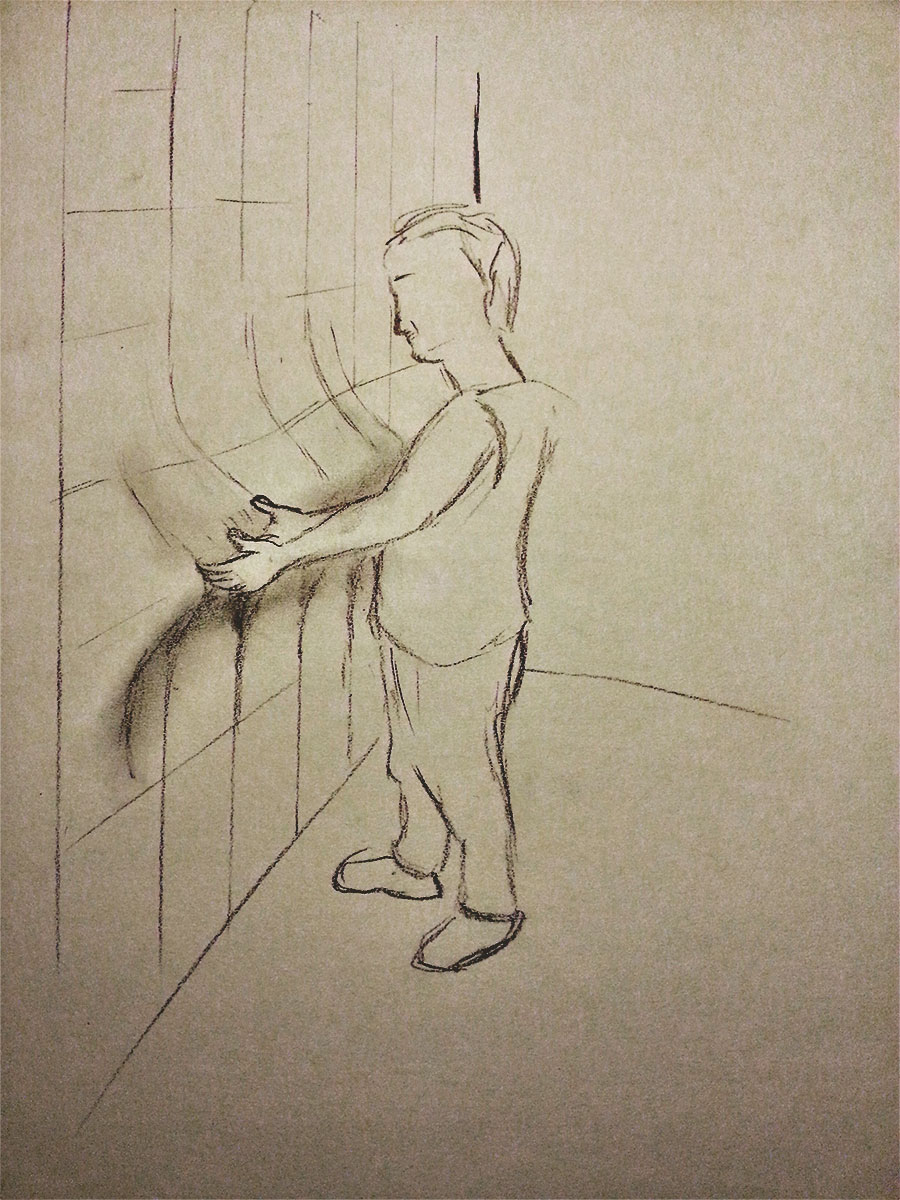
\includegraphics[width=\linewidth]{figures/jamming/concepts/impro/pull}
  \end{subfigure}
  \caption{Sketches of direct deformations of a wall by pushing and pulling, e.g. an improvised shelf.}
\label{fig:ch:jamming:concepts:impro}
\end{figure}



\section{Discussion}

In this chapter we have introduced jamming as an enabling technology for shape changing interfaces.
* types of shape-change

* covered related work - egenskaber og problematikker + hvad vi har laert



\todo{Maybe some Gaver (research through design) and (Alternatives, conceptual design proposals )}
\todo{gentag at SCIs er svaere at konstruere}
\todo{jamming er en interessant approach til AHIs, men andre approaches kunne ogsaa vaere interessante at undersoege}
\todo{jamming er bedst til nogle transformationer, pil til SCI}
\todo{hvad har vi laert ifht AHIs}
